\chapter{Parser mit Yacc und Lex}
Wie bereits gesehen, Programme, die eine CSV-Datei parsen und diese in SQL importieren, gibt es bereits genügend, genauso wie die Möglichkeit da ist, auf Textdateien SQL-Abfragen laufen zu lassen. Außerdem ist auch analysiert worden, welche Bash-Konstrukte bestimmten SQL-Abfragen entsprechen. Darum nun der abschließende Teil der Arbeit - wie können Shell-Skripte geparst und in SQL übersetzt werden.\\

%\begin{figure}
%\centering
%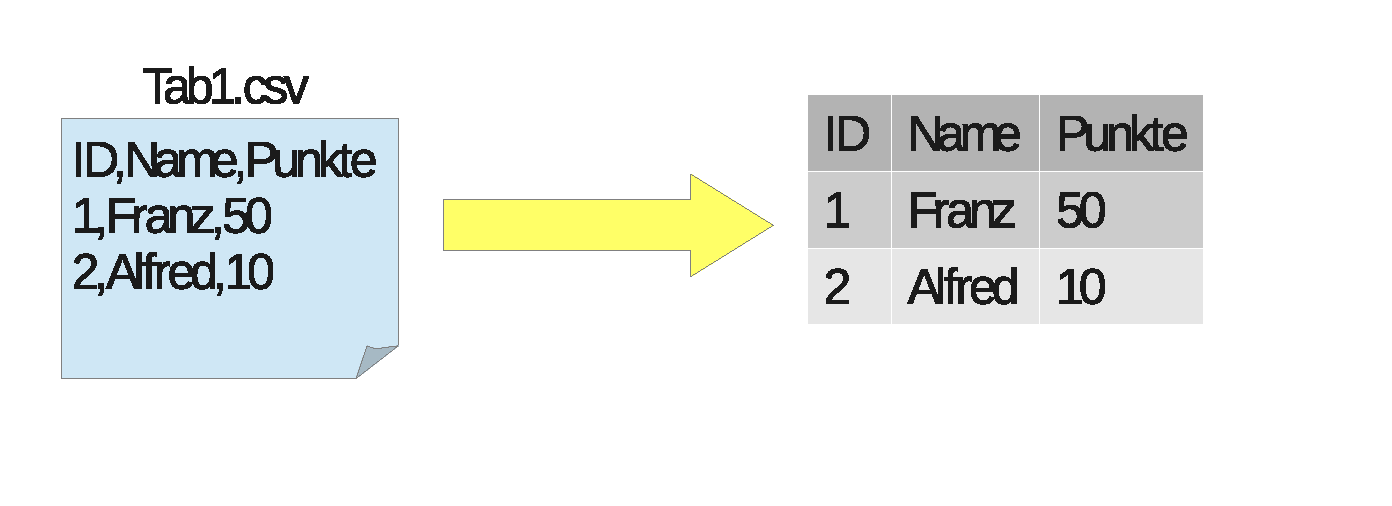
\includegraphics[scale=0.4]{konvert.eps}
%\caption{Import von CSV}
%\label{fig:FigFile}
%\end{figure}

\section{Vorwissen zu Yacc und Lex}
Der erste Versuch verwendet Yacc, ein Programm, das Anfang der 1970-er Jahre von Stephen Curtis Johnson unter dem Namen "'yet another compiler compiler"' für den Compilerbau erfunden und im GNU-Projekt durch Bison ersetzt worden ist. Die Grammatik wird in einer Art Backus-Naur-Form eingegeben, der Parsergenerator Yacc erzeugt dann automatisch ein C-Programm, dass von einer entsprechenden Eingabe liest.\cite{meinders}

%\begin{figure}[h]
%\centering
%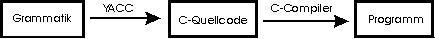
\includegraphics[scale=1]{yacc1.jpg}
%\caption{Arbeitsweise von Yacc nach \cite{meinders} }
%\label{fig:yacc}
%\end{figure}

Wie in Grammatiken üblich, existieren Terminalsymbole, die nicht mehr ersetzt werden, also den endgültigen Symbolen (bei einem Taschenrechner entspricht das den endgültigen Ziffern und Operatoren) und Nichtterminale, also Symbole, die durch Terminale nach bestimmten Regeln ersetzt werden.
Um zu wissen, welche Terminalsymbole verwendet werden, sind zwei Schritte notwendig, zuerst die lexikalische Analyse (welche Symbole kommen vor), die durch die Funktion \lstinline{yylex()} aufgerufen wird und ein Token mit dem gelesenen Symbol zurückgibt, und dem eigentlichen Parser, durch \lstinline{yyparse()} aufgerufen, der anhand der Bausteine die Syntax analysiert und erkennt welche Grammatikregel angewendet wird.
Die Yacc-Quelldatei folgt dabei folgendem Schema:

\begin{lstlisting}
%{
C-Kopf
%}
Yacc-Deklarationen
%%
Grammatiken
%%
/*C-Funktionen, z.B. yylex()*/

int main() {
  reset(queries);
  yyparse();
}
\end{lstlisting}

Für die lexikalische Analyse gibt es zwei Möglichkeiten, entweder man schreibt die Funktion manuell an das Ende oder man nutzt einfach das Programm Lex (oder in der GNU-Version flex), das einem die lexikalische Analyse übernimmt und die Funktion \lstinline{yylex()} automatisch erzeugt. Dazu wird in einer Quelldatei datei.lex angegeben, welche Token bei welchen Symbolen zurückgegeben werden:\cite{meinders}

\begin{lstlisting}
[0-9]+  {yylval = atoi(yytext);
         return NUMBER;}
\end{lstlisting}

Die Kommandos \textit{Lex} und \textit{Yacc} erzeugen, in der Kommandozeile aufgerufen, beide jeweils eine C-Datei (lex.yy.c und y.tab.c), die zum fertigen Parser kombiniert werden.

\begin{lstlisting}
yacc -d parser.y
lex parser.lex
cc -o meinparser lex.yy.c y.tab.c -ll -lm
\end{lstlisting}

Ein einfaches funktionierendes Beispiel findet sich dazu im Anhang.

\section{Der Bash2SQL-Übersetzer mit Yacc}
Das Ziel des Bash2SQL-Übersetzer ist es, ein erstes Erfolgserlebnis zu schaffen und zu zeigen, dass der Weg, ein Shell-Skript in eine SQL-Abfrage zu übersetzen, auch schaffbar ist. Darum behandelt dieser Parser die grundlegende Idee mit vereinfachter Grammatik, die komplette Bash-Grammatik kann erst mit dem nächsten Parser eingelesen werden.
Folglich geht es darum, die Befehle richtig zu übersetzen, also sind zwei Punkte wichtig: Wie wird die SQL-Befehl intern repräsentiert und wie wird ein Komando geparst und übersetzt.
\subsection{Der Quellcode}
Zuerst zum späteren SQL-Befehl, er wird intern als ein einzelner struct abgespeichert, der in Abhängigkeit der eingelesenen Befehle verändert wird. Der struct selbst besitzt nur einige Attribute, ein Feld, um die selektierten Felder als Zahl zu speichern (analog zum Befehl cut und beginnend bei \$1, \$2, usw.) und einen Zeiger auf die nachfolgende Abfrage.

\begin{lstlisting}[language=C]
struct myquery{
        char select[80];
        char from[80];
        char where[800];
        char groupby[20];
        char orderby[20];
        char as[20];
        int felder[MAXFIELDS];

        struct myquery *next;
}
\end{lstlisting}
Da durch das Skript allein nicht zu ermitteln ist, wieviele Spalten die gewählte Tabelle besitzt, wird vorher der Wert \textit{MAXFIELDS} auf eine entsprechend hohe Zahl gesetzt, der die maximale Anzahl an Feldern definiert

\subsection{Der Parser}
Ganz am Anfang erfolgen die Yacc-Deklarationen, also welche Token existieren, und es wird definiert, welche Werte sie zurückgeben. Da nicht nur Strings, sondern manchmal auch Zahlen erwünscht sind, sollen beide Werte möglich sein, die Union-Definition in Kombination mit \textit{\%type} macht es möglich und definiert den Rückgabewert \textit{yylval} als Struktur mit verschiedenen Werten.

\begin{lstlisting}[language=C]
%union {
        long int4;
        int int2;
        float fp; 
        char *str;
};

%type <str> WORD
%type <int4> NUMBER
%type <str> OPT
\end{lstlisting}

Die Typen zu \textit{WORD}, \textit{OPT} und \textit{NUMBER} sind definiert (zu den Grammatiken, die gleich folgen), jetzt fehlen noch die Deklarationen der Token:

\begin{lstlisting}[language=C]
%token  REDIR;
%token  NUMBER ALNUM WORD OPT FSTDIN
%token  PLUS    MINUS   TIMES   DIVIDE  POWER
%token  OPT_D
%token  CAT CUT GREP SORT
%token  PIPE
%token  LEFT_PARENTHESIS        RIGHT_PARENTHESIS
%token  END
\end{lstlisting}

Hinzu kann noch die Bindung und die Priorität der Token festgelegt werden, ersteres durch explizite Angabe, zweiteres implizit durch die Reihenfolge (das letzte bindet am stärksten). Außerdem definiert \textit{\%start} noch explizit das Startsymbol, also die erste anzuwendende Regel der Grammatik, im Folgenden \textit{Input}:

\begin{lstlisting}[language=C]
%left  PIPE
%left   PLUS    MINUS
%left   TIMES   DIVIDE
%left   NEG
%right  POWER

%start Input
\end{lstlisting}

Im dritten Teil können mit den Token Regeln für die Grammatik angegeben werden. Beim Parsen des Kommandos geht es zuerst um die richtige Interpretation der Shell-Kommandos, daher wird zuerst nur eine einfache Shell-Grammatik implementiert. Sie kann aus mehreren Zeilen bestehen und beherrscht auch die Konkatenation mehrerer Kommandos und die Umleitung in eine Datei.

\begin{lstlisting}[language=Bash]
Input:
          /* Empty */
        | Input Line
        ;

Line:
          END
        | Command END                   {
                                                ausgeben(&queries[crtq++]); reset(&queries[crtq]);}
        | Command PIPE Line            
        | Command REDIR WORD END        { strcpy(queries[crtq].as,$3);
                                        ausgeben(&queries[crtq++]);
                                        reset(&queries[crtq]);}
        ;
\end{lstlisting}

Also wie sollen jetzt die Kommandos übersetzt und verbunden werden? Die erste Überlegung ist es, alles in einer SQL-Abfrage abzuhandeln, bis es nicht mehr geht,
also ein \textit{cat tabelle} füttert den From-Teil, ein über Pipe verbundenes \textit{wc -l} füttert die Select-Klausel desselben structs mit einem \textit{count(*)}, am Ende kann die Abfrage ausgegeben werden, also wie folgt:

\begin{figure}[h]
\centering
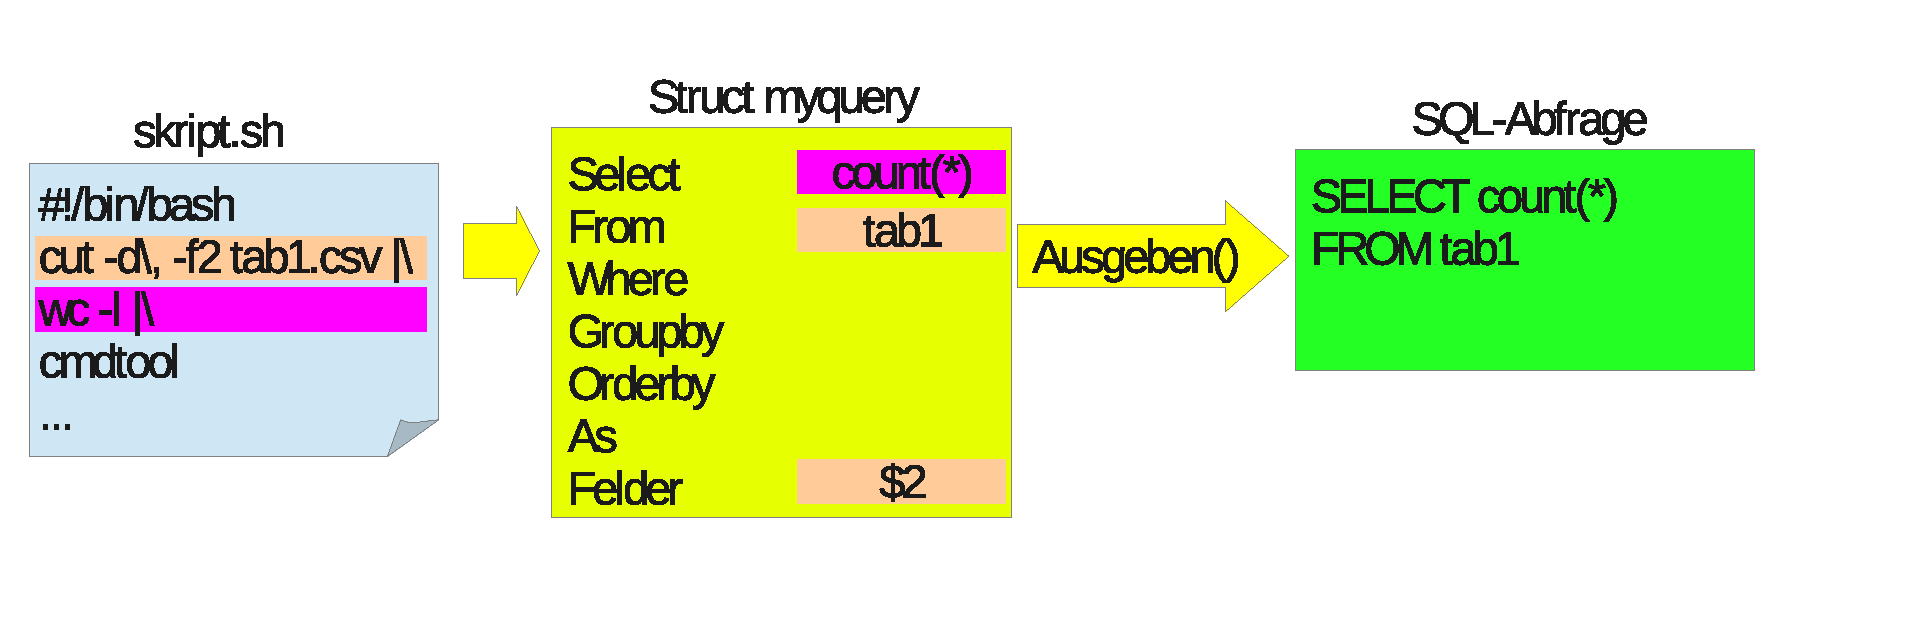
\includegraphics[scale=.4]{parser1.eps}
\caption{Arbeitsweise des Yacc Bash2SQL-Parsers}
\label{fig:parser1}
\end{figure}

Die Idee ist jetzt, für jedes Kommando eine Regel zu erstellen, die in Abhängigkeit des Kommandos (für jedes Kommando ein Token) die Abfrage anders modifiziert.
Außerdem können zu den Kommandos noch Optionen angegeben werden, die beachtet werden müssen, sowie die Eingabedatei, die eingelesen werden soll. Eine Regel der Grammatik besteht immer zuerst aus dem Kommando und dann weiteren Parametern:

\begin{lstlisting}[language=Bash]
<Kommando> [Optionen] Datei [Optionen]
\end{lstlisting}

In dieser Form werden nun die Kommandos geparst, vorläufig werden die Befehle \textit{cat}, \textit{cut}, \textit{grep} und \textit{sort} betrachtet.

\begin{lstlisting}[language=Bash]
Command:
          CAT                           
        | CAT WORD                      { reset(&queries[crtq]);
                                          strcpy(queries[crtq].from,$2);} 
        | CUT OptionsCut WORD           { strcpy(queries[crtq].from,$3);}
                        
        | CUT OptionsCut        
        | GREP WORD             { zugrep(&queries[crtq],$2); }
        | GREP WORD WORD        { strcpy(queries[crtq].from,$3);
                                        zugrep(&queries[crtq],$2); }
        | SORT OptionsSort 
        ;
\end{lstlisting}

Die Aktionen werden entsprechend ausgeführt:
\begin{itemize}
\item \textbf{cat [dateiname]}: der Dateiname ist die gewünschte CSV-Datei und entspricht dem Tabellennamen, also kann der Name so in die From-Klausel übernommen werden (\lstinline{strcpy(queries[crtq].from, $2)})
\item \textbf{cut Optionen [dateiname]}: wieder ist der Dateiname (sofern angegeben) die gewünschte Tabelle, die Optionen werden mit einer eigenen Regel extra geparst
\item \textbf{grep Muster [Dateiname]}: wieder analog, nur dass ein Muster angegeben ist, also ein Prädikat. Die Funktion \lstinline{zugrep()} erzeugt eine Bedingung die in jeder Spalte nach Vorkommen des Musters sucht
\item \textbf{sort Optionen}: eigene Regel für die Optionen
\end{itemize}

\subsection{Der Lexer}
Die Token liefert lex, der für die lexikalische Analyse zuständig ist. Der erhält die deklarierten Token und die Definition der Kommunikationsvariable \textit{yylval} in den Anfangsdefinitionen:
\begin{lstlisting}
%{
#include "y.tab.h"
extern YYSTYPE yylval;
#include <stdio.h>
#include <stdlib.h>
%}
\end{lstlisting}

Anschließend folgt eine Definition über die Arten von Symbolen, welche vorkommen können.
\begin{lstlisting}
white           [ \t]+

digit           [0-9]
integer         {digit}+
exponant        [eE][+-]?{integer}

real            {integer}("."{integer})?{exponant}?

letter          [a-zA-Z0-9\.\,\|]+

options         -[a-zA-Z0-9\-\,]+\ 
ende            [^\\];
\end{lstlisting}
Mit \textit{\%\%} wird der Beginn der syntaktischen Analyse gekennzeichnet, auch als lex-Regeln bekannt, die die Token liefern, also die Terminalsymbole für Yacc.
Leerzeichen und Tabulatoren sollen ignoriert, bei Zahlen soll ein Integer-Wert zurückgegeben werden, also das Attribut int4 von yylval, bei Zeichenketten ein String und für jeden Befehl soll ein eigenes Token produziert werden.
\begin{lstlisting}
{white}         {  }
{real}          {
                  yylval.int4=atoi(yytext);
                  return(NUMBER);
                }
">"             return(REDIR);
"|"             return(PIPE);
"cat"           return(CAT);
"cut"           return(CUT);
...

"\n"            return(END);
{letter}        {
                        yylval.str=strdup(yytext);
                        return WORD;
                }
\end{lstlisting}
Aus diesen Regeln generiert Lex nun die Funktion yylex(), die bei jedem Aufruf Zeichen einliest, bis sie ein Token zurückgibt. Im Zusammenspiel mit Yacc ruft dieser yyparse(), die yylex() benutzt und anhand der zurückgegebenen Token erkennt, ob die Eingabe richtig ist.

\subsection{Bedienung des Bash2SQL-Übersetzers}
Im Ordner \textit{bash\_parser\_yacc} liegen die Dateien \textit{bash2sql.lex} und \textit{bash2sql.y}, also die Lexer-Regeln und die Yacc-Grammatik. Das beiliegende Makefile kompiliert aus den Dateien das Programm \textit{kleinerParser} (s. Abb, \ref{fig:lexyacc}), das aus einfachen Shell-Skripten SQL-Abfragen erzeugt.

\begin{figure}[h]
\centering
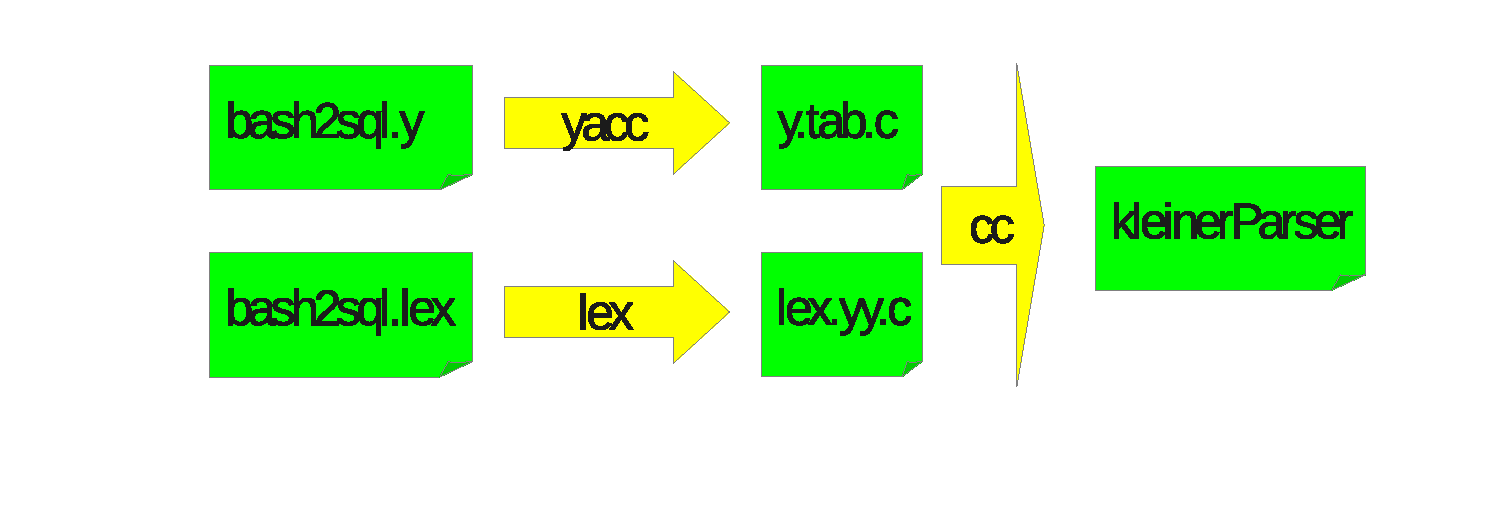
\includegraphics[scale=.4]{yacc.eps}
\caption{Zusammenspiel von Lex und Yacc}
\label{fig:lexyacc}
\end{figure}

Der Übersetzer arbeitet als einfacher Filter, er liest von der Standardeingabe und gibt auf der Standardausgabe das Ergebnis aus. Ein Befehl kann direkt übersetzt werden.

\begin{lstlisting}[language=Bash]
$ echo "cat tabelle | cut -f1,2,3 | grep Muster" | ./kleinerParser
\end{lstlisting}

Oder ein Befehl wird aus einer Datei gelesen.
\begin{lstlisting}[language=Bash]
$ cat abfrage.sh | ./kleinerParser
\end{lstlisting}

In beiden Fällen wird folgende Ausgabe erzeugt:
\begin{lstlisting}[language=Bash]
SELECT $1,$2,$3, FROM tabelle WHERE ($1 like '%Muster%'
	or $2 like '%Muster%' or $3 like '%Muster%' 
	or false) GROUP BY  ORDER BY  AS
\end{lstlisting}

Da die Spaltennamen noch nicht eingelesen werden, müssen sie noch manuell ersetzt werden. Bis auf ein paar Schönheitsfehler ist die Abfrage in Ordnung.

\chapter{Parser mit ANTLR}
Der bisherige Parser unterstüzt nur sehr wenige Befehle, implementiert noch die gesamte Shell-Grammatik und bedarf einiger Korrekturen um korrekte SQL-Syntax zu erzeugen. Dabei lohnt sich gleich der Umstieg auf einen mächtigeren Parser-Generator, der außerdem den Code in verschiedenen Programmiersprachen erzeugen kann, nämlich der Parser-Generator \textbf{ANTLR}.
\section{Konfiguration}
Der ANTLR-Parser basiert auf Java und erzeugt ohne Erweiterung nur Parser in dieser Sprache, soll der Parser für andere Sprachen Quelldateien ausspucken, so ist eine Bibliothek zu installieren.

\subsection{Installieren der Bibliothek}
Für einen Parser in C/C++ wird die Bibliothek \textit{libantlr3c-3.4 }
\footnote{\label{foot:1}erhätlich unter \url{http://www.antlr3.org/download/}}
benötigt, sie enthält alle benötigten Funktionen bzw. Klassen.
Die Datei herunterladen, entpacken, konfigurieren und installieren. Dabei ist folgendermaßen vorzugehen:
\begin{lstlisting}[language=Bash]
tar -xzf libantlr3c-3.4.tar.gz
cd libantlr3c-3.4
./configure --enable-64bit
make
make install
\end{lstlisting}
Läuft das Programm auf einem 32-Bit-System, so ist der dritte Schritt durch \textit{./configure} zu ersetzen. Anschließend ist die Bibliothek in \textit{/usr/local/lib} installiert.

\subsection{Starten von ANTLR}
Zuerst muss der Parsergenerator als \textit{antlr-3.5.2-complete.jar} \ref{foot:1} heruntergeladen werden, aber in der Version 3.5.2, da neuere Versionen noch nicht die Codegenerierung in andere Sprachen beherrschen.
Für den folgenden Schritt wird angenommen, dass die jar-Datei in \textit{~/Downloads} liegt.
Bevor der Parser-Code generiert werden kann, muss der Klassenpfad für Java und der Pfad zur Bibliothek gesetzt werden, damit die Java Virtual Machine die Komponenten von ANTLR findet und die Bibliothek eingebunden ist.
\begin{lstlisting}[language=Bash]
export LD_LIBRARY_PATH=/usr/local/lib:$LD_LIBRARY_PATH
export CLASSPATH=~/Downloads/antlr-3.5.2-complete.jar:$CLASSPATH
\end{lstlisting}

\subsection{Vorwissen zu ANTLR}
Im Gegensatz zu anderen Parsern ist ANTLR in einer objektorientierten Sprache geschrieben (wie schon erwähnt in Java), so realisiert er Lexer und Parser als zwei verschiedene Klassen. ANTLR ist mächtiger als Yacc mit Lex, da die lexikalische Analyse auch kontextsensitive Grammatiken unterstützt, LEX nur kontextfreie.
Außerdem ist es in ANTLR möglich, die Regeln für die lexikalische und grammatikalische Analyse in eine Grammatik-Datei zu packen, können aber - dank Modularität - auf mehrere aufgeteilt werden. Die Dateien enden auf \textit{.g} und folgen dem Schema:\cite{antlr}
\begin{lstlisting}
<Grammatik-Typ> grammar <name>;
<Optionen>
<Token-Definition>
<Quellcode>
<Grammatik-/Lexer-Regeln>
\end{lstlisting}

In den Bereich für den Quellcode können sowohl die Kopfzeilen und Deklarationen, wie auch die Funktionen angegeben werden, der Teil kombiniert also den zweiten und letzten Bereich des Schemas von Yacc, dennoch sind sie mit einem Schlüsselwort voneinander abzugrenzen:
\begin{lstlisting}
@header
{
/* Parser-Kopf */
}
@members
{
/*  Parser-Rumpf */
}
\end{lstlisting}

Die Lexer-Definitionen erfolgen analog durch die Schlüsselworte \textit{@lexer::header} und \textit{@lexer::members}. Die anderen Teile stehen für Folgendes:
\begin{enumerate}
\item <Grammatik-Typ> entweder Lexer, Parser oder AST, fehlt die Angabe, so Lexer und Parser kombiniert
\item <Optionen> unter anderem die Zielsprache
\item <Token-Definition> und <Quellcode> sind analog zu Yacc und Lex
\item <Grammatik-/Lexer-Regeln> sind die gewünschten Regeln
\end{enumerate}
Ein schönes und einfaches Beispiel findet sich auf der Homepage \url{www.antlr.org}, im Nachfolgenden werden nur die Zielsprachen C/C++ betrachtet.

\section{Der Bash2SQL-Übersetzer mit ANTLR in C}
Dieses Mal soll die komplette Bash-Grammatik geparst werden können, die Abfragen sollen modularer und syntaktisch korrekt aufgebaut sein und mittels ANTLR für C generiert. Die Zielsprache ist C und das wird in den Optionen mitgeteilt und noch ein kleiner Bugfix im Kopf des Lexers:

\begin{lstlisting}
options
{
    language=C;
}

tokens
{
    PIPE = '|';
}

@lexer::header
{
/* ein Fix wenn Zustand _empty nicht deklariert*/
#define _empty NULL
}
\end{lstlisting}

\subsection{Neues Konzept}
Bisher sind die Kommandos der Reihe nach geparst und in eine SQL-Abfrage übersetzt worden, bis es nicht mehr geht, wenn ein Kommando unbekannt ist. Jetzt ist die Überlegung, dass jedes Kommando für sich allein steht und eine eigene SQL-Abfrage ergibt. Die Ausgabe erfolgt über den Standardfluss, kann also mit weiteren Kommandos durch eine Pipe verbunden werden. So können auch die einzelnen, bereits ausgeführten, SQL-Abfragen verbunden werden, indem das modfizierte Skript die Ausgabe durchreicht (s. Abb. \ref{fig:parser2}).

\begin{figure}[h]
\centering
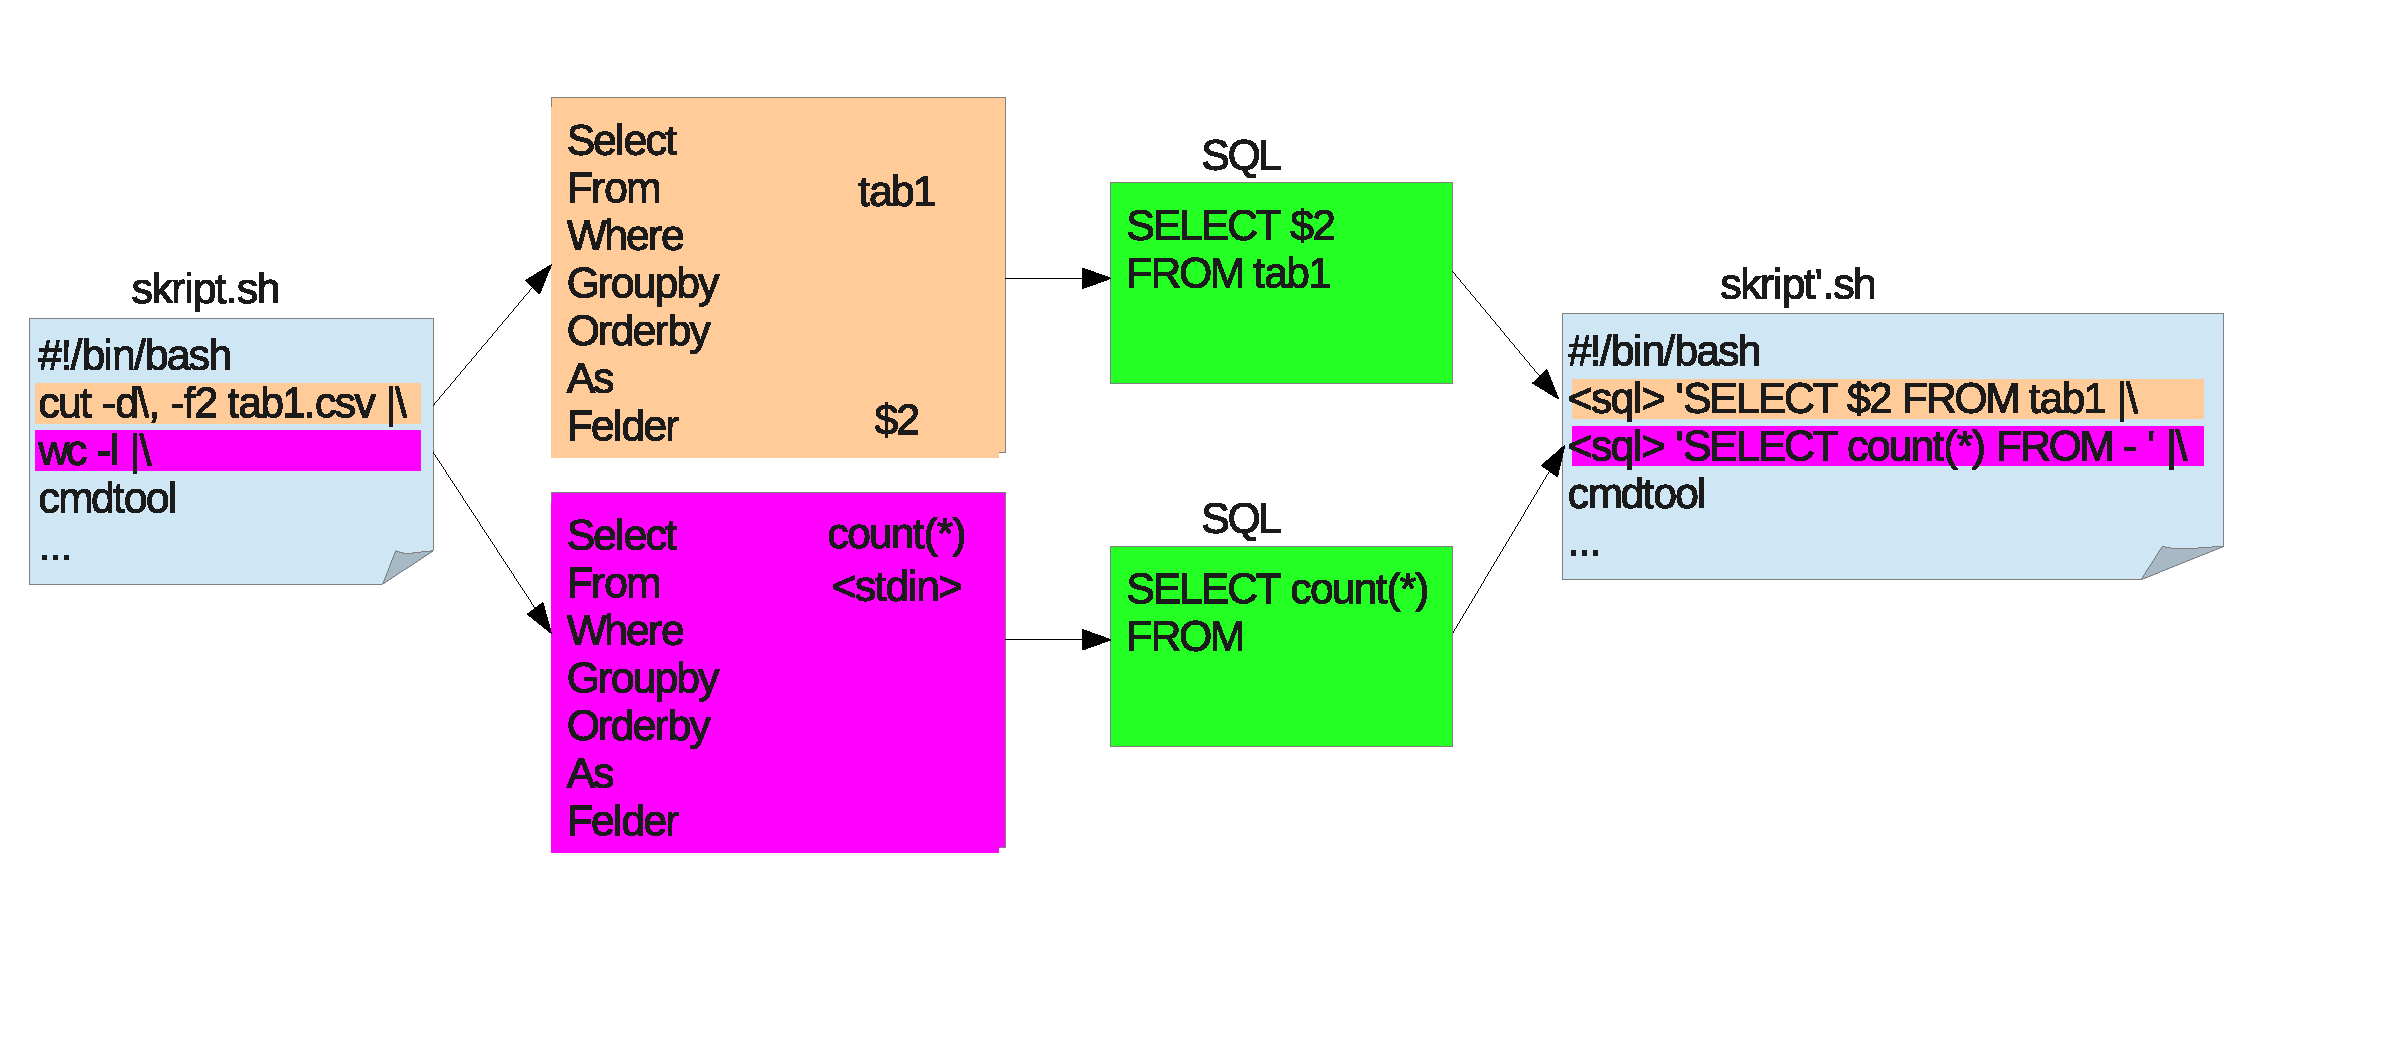
\includegraphics[scale=.4]{parser2.eps}
\caption{Neues Konzept}
\label{fig:parser2}
\end{figure}

Schöner ist es natürlich, wenn der Übersetzer gleich erkennt, wann er welche Abfragen zusammenfügen kann, sodass am Ende eine geschachtelte SQL-Abfrage entsteht, die auch optimiert werden kann. Das ist besser, als wenn jede Abfrage einzeln ausgewertet wird und die Kommunikation mit Hilfe der Shell erfolgt, die die Daten über den Strom schickt. Die vorgestellte Idee wird modifiziert, indem der Parser solange die Kommandos liest, bis er am Ende ist oder ein ihm unbekanntes Kommando erscheint. Für jedes gelesene Kommando wird eine Abfrage erstellt, die die vorherige, falls existent, als Quelltabelle aufnimmt. Daraufhin entsteht eine geschachtelte SQL-Anweisung. Im Moment steht diese dann zwischen allen nicht erkannten Kommandos, sodass ein wieder funktionierendes Skript erzeugt wird (s. Abb. \ref{fig:parser3}).

\begin{figure}[h]
\centering
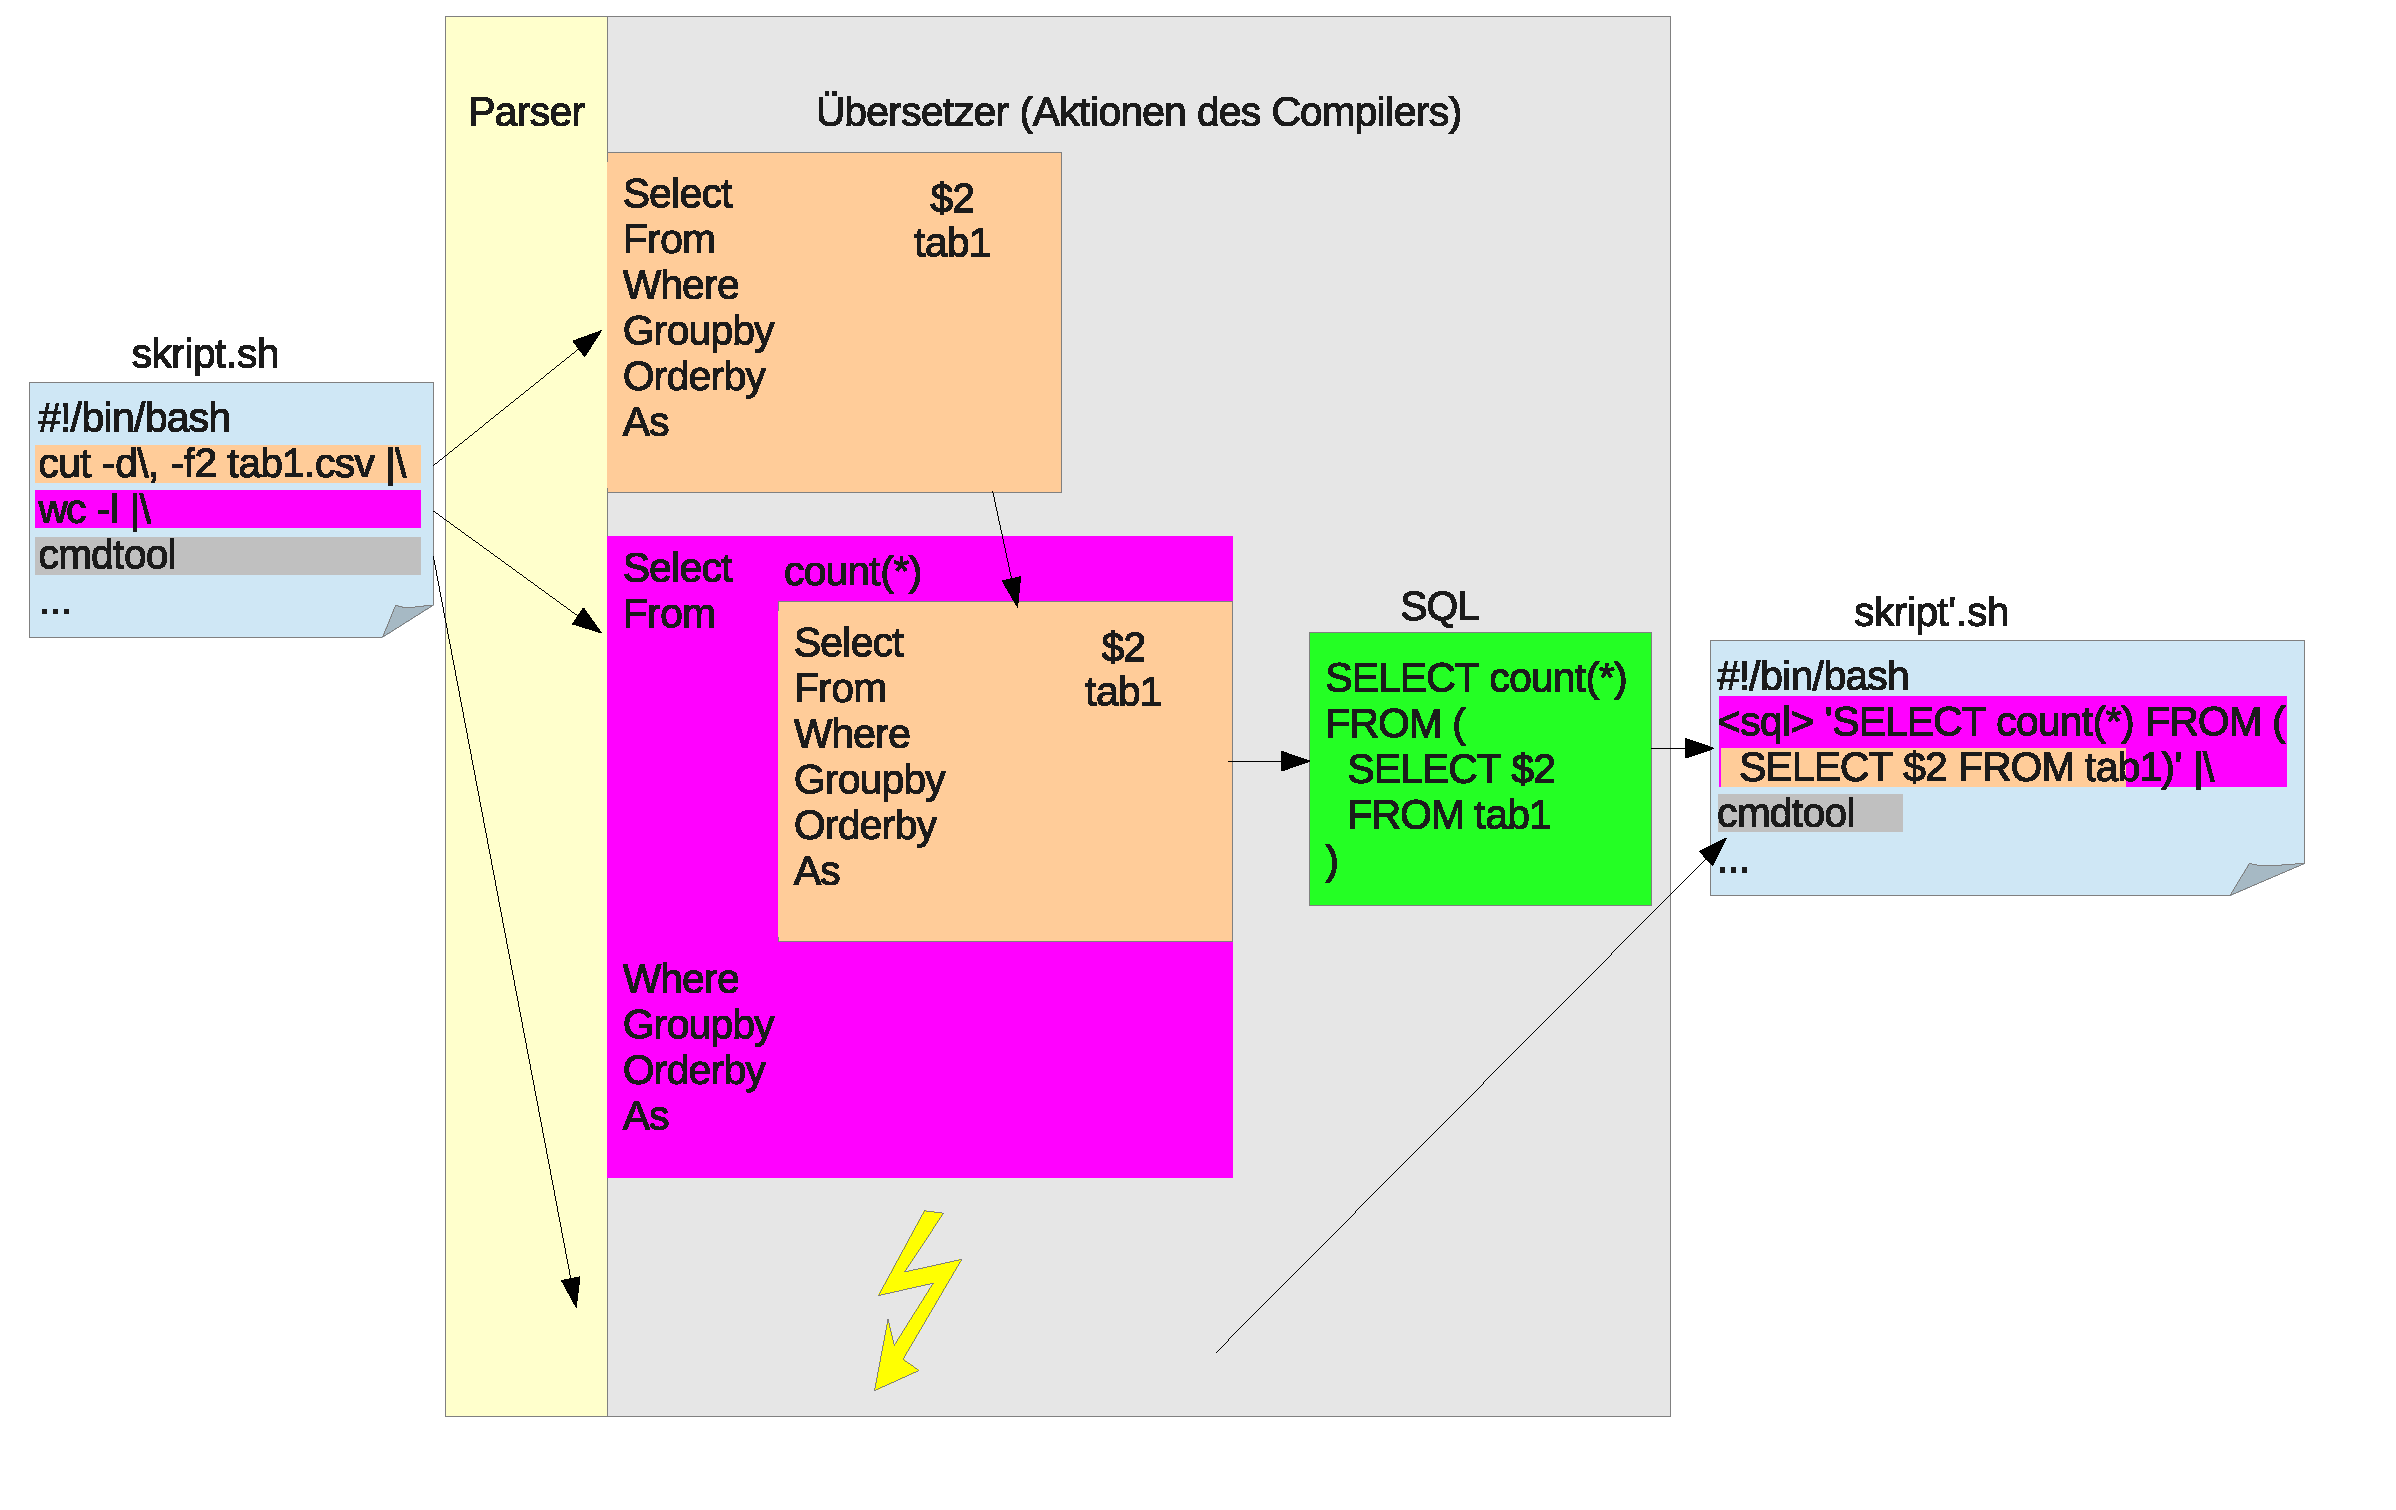
\includegraphics[scale=.4]{parser3.eps}
\caption{Neues Konzept mit Schachtelung}
\label{fig:parser3}
\end{figure}

\subsection{C-Quellcode}
Um wieder dem Schema einer Grammatikdatei zu folgen, werden zuerst die Definitionen des C-Quellcodes beschrieben.
Im Grunde ist die Definition des SQL-Abfrage-Structs, die auch den gesamten Parser-Kopf bildet, identisch zu der des Parsers in Yacc, lediglich einige Erweiterungen um Joins und Vereinigungen zu bilden sind hinzugegekommen.

\begin{lstlisting}[language=C]
@header
{
#ifndef MYHEAD
#define MYHEAD

 #include <assert.h>
 #include "SimpleBashSQLLexer.h"
 #define MAXFIELDS 5
 #define DELIMIT ','

 typedef struct myquery{
        char select[10], from[30],
        where[200], groupby[5],
        orderby[5], as[20];
        /*numerische Repraesentation der Felder*/
        char felder[MAXFIELDS], groups[MAXFIELDS], orders[MAXFIELDS];
        /*sprechende Namen */
        char *fname[MAXFIELDS];
        /* findet join statt? felder 1, felder2, tabelle1, tabelle2 */
        char join, f1,f2,t2[20];
        /* findet union statt?  */
        char sqlunion,sort,group,nrfields;
        struct myquery *src, *src2;
  } query;


#endif
}
\end{lstlisting}

Desweiteren werden noch, um den struct bearbeiten zu können, einige Funktionen benötigt, die sich im Detail im Anhang finden und für folgende Aufgaben zuständig sind:

\begin{itemize}
\item int lookup(char* filename, char delimit,query *q): liest die erste Zeile einer Datei und nimmt die Werte als Spaltenbezeichner für die gewünschte Abfrage
\footnote{das Teilen einer Zeichenkette erfolgt frei nach \cite{split}}
\item int reset(query* abfrage): initialisert einen struct, entspricht einem Konstruktor
\item int deletequeries(query* q): gibt Speicherplatz frei, entspricht Destruktor
\item int ausgeben(query* e): gibt einen struct query als SQL-Abfrage aus
\item query *makeunion(char* eingabe, query* q) bzw. query *makeunion\_query(query* eingabe, query* q): bilden die Vereinigung aus mehreren Tabellen, im ersten Fall mittels eines Tabellennamens, im zweiten mittels einer weiteren Abfrage
\item int zugrep(char* pattern, query* abfrage): erzeugt aus einem Suchmuster das passende Prädikat für die Where-Klausel
\item int parseListe(char*e, char* feld): nimmt die Spaltenangaben, wie sie in der Shell üblich sind, und selektiert aus einem Feld nur die gewünschten
\item int opts<cmd>(char* e, query* q):
parst die Optionen zu dem jeweiligen Kommando <cmd>
\end{itemize}

Damit der ANTLR-Parsergenerator laufen kann, muss die Main-Methode stimmen. Deren Aufbau wird zwar in verschiedenen Foren erklärt, nur leider sind die meisten Erklärungen veraltet und beziehen sich auf ältere Versionen des Parsergenerators. \cite{ANTLR-C}
\begin{enumerate}
\item Im Gegensatz zu Yacc liest ein ANTLR-Parser die Eingabedatei als Operand ein: \lstinline{argc==2}, sonst breche ab
\item die Funktion, die den Lexer füttert, ist zu ersetzen durch: \lstinline{antlr3FileStreamNew ((pANTLR3_UINT8)argv[1], ANTLR3_ENC_8BIT);}
\item zuletzt noch das Startsymbol für die Grammatik festlegen, hier \textit{file}: \lstinline{parser->file(parser);}
\end{enumerate}
Zusammengesetzt mit den übrigen Funktionen sieht das dann so aus:

\begin{lstlisting}[language=C]
int main(int argc, char * argv[])
{
	pANTLR3_INPUT_STREAM           input;
	pSimpleBashSQLLexer            lex;
	pANTLR3_COMMON_TOKEN_STREAM    tokens;
	pSimpleBashSQLParser           parser;

	if(argc!=2){
		printf("\%s: fehlender Operand\n",argv[0]);
		return 1;
	}

	input = antlr3FileStreamNew (
		(pANTLR3_UINT8)argv[1], ANTLR3_ENC_8BIT);
	lex    = SimpleBashSQLLexerNew                (input);
	tokens = antlr3CommonTokenStreamSourceNew
		(ANTLR3_SIZE_HINT, TOKENSOURCE(lex));
	parser = SimpleBashSQLParserNew               (tokens);

	parser  ->file(parser);

	parser ->free(parser);
	tokens ->free(tokens);
	lex    ->free(lex);
	input  ->close(input);

	return 0;
}
\end{lstlisting}

Die Konfiguration ist fertig, jetzt kann mit den Grammatik-Regeln begonnen werden. Zuerst muss natürlich die Shell-Grammatik implementiert sein, praktischerweise existieren zahlreiche Bücher, die die Grammatik in Backus-Naur-Form beschrieben haben und sich somit leicht in ANTLR importieren lässt. \cite{Shell-BNF}

\subsection{Die Grammatik}
Besonders interessant ist die Stelle, dir für die Ausgabe der SQL-Anweisung zuständig ist, die Regel \textit{pipeline\_cmd}. Sie erkennt die Konkatenation meherere Befehle (\textit{command}) mittels einer Pipe. Die Kommunikation erfolgt über eine Referenz auf den letzten SQL-Abfrage-Struct \textit{lastquery}, ist dieser \textit{NULL}, so konnte das Kommando nicht geparst werden und der Befehl soll wieder ausgegeben werden. Alternativ wird am Ende der SQL-Abfrage-Struct ausgegeben. Das Attribut \textit{tobeprint} dient zum Erkennen, ob zuerst der Kopf einer Schleife ausgegeben werden soll.

\begin{lstlisting}
pipeline_cmd    : c1=command
                        {
                        if(tobeprint && !lastquery && $c1.text->chars)
                                printf("\%s",$c1.text->chars);
                        }
                (PIPE c2=command
                        {
                        if(tobeprint && !lastquery)
                                printf(" | \%s",$c2.text->chars);
                        }
                )*
                {
                if(lastquery)
                        ausgeben(lastquery);
                printf("\n");
                tobeprint=1;
                }
        ;
\end{lstlisting}

Auf diese Weise steigt man ab bis zur Regel \textit{cmd}.
\begin{lstlisting}
cmd returns [query *r]
\end{lstlisting}
Am Anfang wird Platz für einen neuen Query-Struct geschaffen, der als Quelle den vorherigen erhält (\textit{lastquery}):
\begin{lstlisting}
@init{
        /* neue Query r, vorherige Abfrage als FROM-Tabelle
                NULL, wenn erstes Kommando */
        char tmp=0; //zaehlt args
        r=(query*) malloc(sizeof(query));
        r->src=lastquery;
        reset(r);
}
\end{lstlisting}
Am Ende ist die aktuelle Query die letzte, also:
\begin{lstlisting}
@after{
        lastquery=r;
}
\end{lstlisting}
Da das Parsen der Befehle und das Ausführen der zugehörigen Aktionen meistens sehr ähnlich abläuft, wird nachfolgend das Erkennen von \textit{cut} vorgestellt.\\
Zuerst wird immer der Befehl geparst, anschließend die Parameter. Der Zugriff auf den Inhalt eines Symbols erfolgt mit \lstinline{\$SYMBOL.text->chars} als Zeichenkette (char*):
\begin{lstlisting}
  'cut'         ( OPTS
			{ optscut($OPTS.text->chars,r); }
		| WORD
			{ r=makeunion($WORD.text->chars,r); }
		| from_redir
			{/* fname!=NULL, wenn Dateiname */
			if ($from_redir.fname)
				r=makeunion($from_redir.fname,r);
			else /* sonst subshell */
				r=makeunion_query(lastquery,r);
			}
		| '- ' )+

\end{lstlisting}
Als Parameter können Optionen oder die anzuzeigende Datei angegeben werden. Optionen (das Lexer-Token \textit{OPTS}) werden mit der Methode \textit{optscut()} gleich analysiert und das Ergebnis in den Struct eingebunden. Für jedes Kommando existiert eine eigene Funktion, um die Optionen zu parsen, also die eine Zeichenkette nimmt und sie Buchstabe für Buchstabe abarbeitet.
\begin{lstlisting}[language=C]
/* zu cut */
int optscut(char* e, query* q){
	/*bis Ende erreicht*/
	while(*++e!=0){
		switch (*e){
		case 'f':
			parseListe(e,q->felder);
			break;
		}
	}
	return 1;
}
\end{lstlisting}
Da mit der Option \textit{-f} die auszugebenden Spalten bezeichnet sind, wird die Funktion \lstinline{parseListe()} benötigt, die mithilfe einer solchen Kette die gewünschten Felder extrahiert, bei \textit{cut} also die zu selektierenden Felder.

\begin{lstlisting}[language=C]
int parseListe(char*e, char* feld)
{
	int crtf=0;
	int a,b,ret;
	do{
		e++;
		ret=sscanf(e,"\%d-\%d",&a,&b);
		/* felder beginnen bei 0*/
		a--; b--;
		if(ret==0)/*error*/
			return -1;
		/* von - bis  */
		else if(ret==2){
			for(;a<=b;a++)
			   feld[crtf++]=feld[a];
		}/*einzelne Auswahl */else{
			feld[crtf++]=feld[a];
		}
		while((*e>='0' && *e<='9')||*e=='-')
			e++;
	}while(*e==',');
	feld[crtf]=-1;
	return 1;
}
\end{lstlisting}
Mit den vorgestellten Methoden und Regeln ist es nun möglich, komplette Bash-Skripte zu parsen und die unterstützten Kommandos zu interpretieren.

\subsection{Lexer-Regeln}
Der Vollständigkeit halber seien hier auch noch die Regeln zur syntaktischen Analyse beschrieben. Diese befinden sich bei ANTLR bei den übrigen Regeln, aus Konvention werden diese Symbole, die durch Terminale zu ersetzen sind, jedoch großgeschrieben.

\begin{lstlisting}
/*------------------------------------------------------------------
 * LEXER RULES
 *------------------------------------------------------------------*/
OPTS            : ('-'|'+') (LETTER|DIGIT|'-')+
                ;
NUMBER          : (DIGIT)+
                ;
WORD            : (LETTER|DIGIT)+;
ALCHAR          : (LETTER|NUMBER|SONDER)+;
WHITESPACE      : ( '\t' | ' ' | '\r' | '\u000C' | '\\' '\n' | '"')+
                {
                         $channel = HIDDEN;
                }
                ;
fragment
DIGIT           : '0'..'9';
fragment
LETTER          : ('A'..'Z'|'a'..'z'|'.'|'_'|','|'\|' | '\;'|'$');
fragment
SONDER          : ('{' | '}' | '%' | '\'' | '`' | '-' | '=' | '/' | '!' );
\end{lstlisting}


\subsection{Bedienung}
Im Ordner \textit{c\_bash\_parser\_Yacc} liegen die Grammatikdatei \textit{SimpleBashSQL.g} und ein Makefile. Beide reichen aus, um mit \textit{make} den Parser zu erzeugen, wenn die Bibliothek richtig installiert und die Pfade richtig gesetzt sind.\\
ANTLR erzeugt eine Lexer- und eine Parser-Quelldatei \textit{SimpleBashSQL\{Lexer,Parser\}.\{h,c\}}, die zu dem fertigen Compiler mittels \textit{cc} kompiliert werden:

\begin{lstlisting}[language=make]
all: simplebashsql

simplebashsql: $(OBJ).g
        java org.antlr.Tool $^
        gcc -g -o $@ -I/usr/local/include/ -L/usr/local/lib/ -lantlr3c $(OBJ)Parser.c $(OBJ)Lexer.c
\end{lstlisting}

Das Programm nimmt den Dateinamen eines Skripts als Eingabeparameter und schickt das Ergebnis auf die Standardausgabe. So wird das Skript:
\begin{lstlisting}[language=Bash]
#!/bin/bash
cut -f1,2,3 vorlesungen.csv | sort -k2
\end{lstlisting}
übersetzt in:
\begin{lstlisting}
#!/bin/bash
SELECT VorlNr,Titel,SWS FROM  (
	SELECT VorlNr,Titel,SWS FROM vorlesungen.csv AS b
) AS b ORDER BY $1 
\end{lstlisting}

\section{Der Bash2SQL-Übersetzer mit ANTLR in C++}
So schön die Sprache C auch ist, so ist die Speicherverwaltung mit ihr ziemlich anstrengend, vor allem da die Bezeichner von Tabellen oder Spalten unterschiedlich lang werden können, lohnt sich der Umstieg auf C++ mit impliziter Speicherverwaltung und einer Standardbibliothek mit \textit{vector} und \textit{string}, die einem das Leben erleichtern. Außerdem kann ein höheres Abstraktionsniveau erreicht werden, indem die Abfrage über eine eigene Klasse gekapselt wird und der Zugriff nur noch über Methoden erfolgt und Änderungen nicht mehr per Hand durchgeführt werden müssen.

\subsection{Unterschiede: C vs. C++ mit ANTLR}
Um ANTLR C++-Code generieren zu lassen, sind einige Änderungen nötig.

Die Unterstützung von C++ in ANTLR baut auf sogenannten Traits auf, also vorgefertigten Klassen die in ähnlicher Weise wiederverwendet werden, in dem vorliegenden Fall für den Lexer.

\begin{lstlisting}[language=C++]
@lexer::traits {
     class  SimpleBashSQLLexer;
     class  SimpleBashSQLParser;
     typedef antlr3::Traits< SimpleBashSQLLexer, SimpleBashSQLParser > SimpleBashSQLLexerTraits;
     typedef SimpleBashSQLLexerTraits SimpleBashSQLParserTraits;
}
\end{lstlisting}

Die Header-Dateien, in denen die verwendeten Klassen wie \textit{antlr3} definiert sind, müssen zum Kompilieren eingebunden werden. Die Dateien finden sich im \textit{antlr3-master} (erhätlich bei github
\footnote{\url{https://github.com/antlr/antlr3}})
im Verzeichnis \textit{antlr3-master/runtime/Cpp/include}.

Die Main-Methode muss natürlich auch noch verändert werden, die Funktionsweise ist aber identisch zum Parer in C, die einzulesende Datei wird als Operand mitgegeben.

\begin{lstlisting}[language=C++]
int main(int argc, char * argv[])
{
	if(argc!=2){
		printf("\%s: fehlender Operand\n",argv[0]);
		return 1;
	}

	ANTLR_UINT8* fName = (ANTLR_UINT8*) argv[1];
	SimpleBashSQLLexer::InputStreamType input(fName, ANTLR_ENC_8BIT);
	SimpleBashSQLLexer lxr(&input); // TLexerNew is generated by ANTLR
	SimpleBashSQLParser::TokenStreamType tstream(ANTLR_SIZE_HINT, lxr.get_tokSource() );
	SimpleBashSQLParser psr(&tstream); // TParserNew is generated by ANTLR3
	psr.file();
	return 0;
}
\end{lstlisting}

Um in den Aktionen auf den Wert eines Symbols zugreifen zu können, dienen Ströme (Streams). Soll der Wert ausgegeben werden, so erfolgt der Zugriff über das Attribut \textit{text}, zum Beispiel eine Ausgabe auf der Standardausgabe:
\begin{lstlisting}[language=C++]
comment { std::cout << $comment.text; }
\end{lstlisting}
Soll der Inhalt in eine Zeichenkette überführt werden, so ist der Umweg über einen \textit{stringstream} praktisch, da die Methode \lstinline{str()} einen String zurückgibt. 

Der Tokenstream funktioniert nur mit Nichtterminalsymbolen (Parserregeln), das heißt für jede Lexerregel, also die, die auf Terminalen arbeiten, muss eine Parserregel existieren. So besteht eine Zahl (\textit{NUMBER}) aus Ziffern (\textit{DIGIT}), dazu muss noch eine Parserregel \textit{number} erstellt werden, um die zugehörige Zeichenkette, also die Zahlen, auszugeben:
\begin{lstlisting}
number: NUMBER;
NUMBER          : (DIGIT)+
                ;
fragment
DIGIT           : '0'..'9';
\end{lstlisting}
Die letzte Regel ist als \textit{fragment} gekennzeichnet, da Ziffern immer als Teil einer Zahl vorkommen sollen, keine Parserregel darf darauf aufbauen.

\subsection{Die Klasse TheQuery}
Für die erste fundamentale Änderung werden alle Operationen für eine Abfrage in der Klasse \textit{TheQuery} gekapselt. Alle Veränderungen am Datenbestand erfolgen jetzt über Methoden, die interne Repräsentation interessiert den späteren Compiler nicht und das Praktische daran: die Klasse steht für sich allein und ist auch komplett austauschbar durch ein Substitut, das nur die entsprechenden Schnittstellen implementieren muss.
Bevor die Methoden betrachtet werden, sollte sich der Aufbau der Klassen überlegt werden. Um einen praktikablen SQL-Standard zu erfüllen, orientiert sich der Aufbau an der DB2-Referenz von IBM, der schön modular beschrieben ist \cite{db2}.

\subsubsection{Interne Repräsentation}
\begin{figure}[h]
\centering
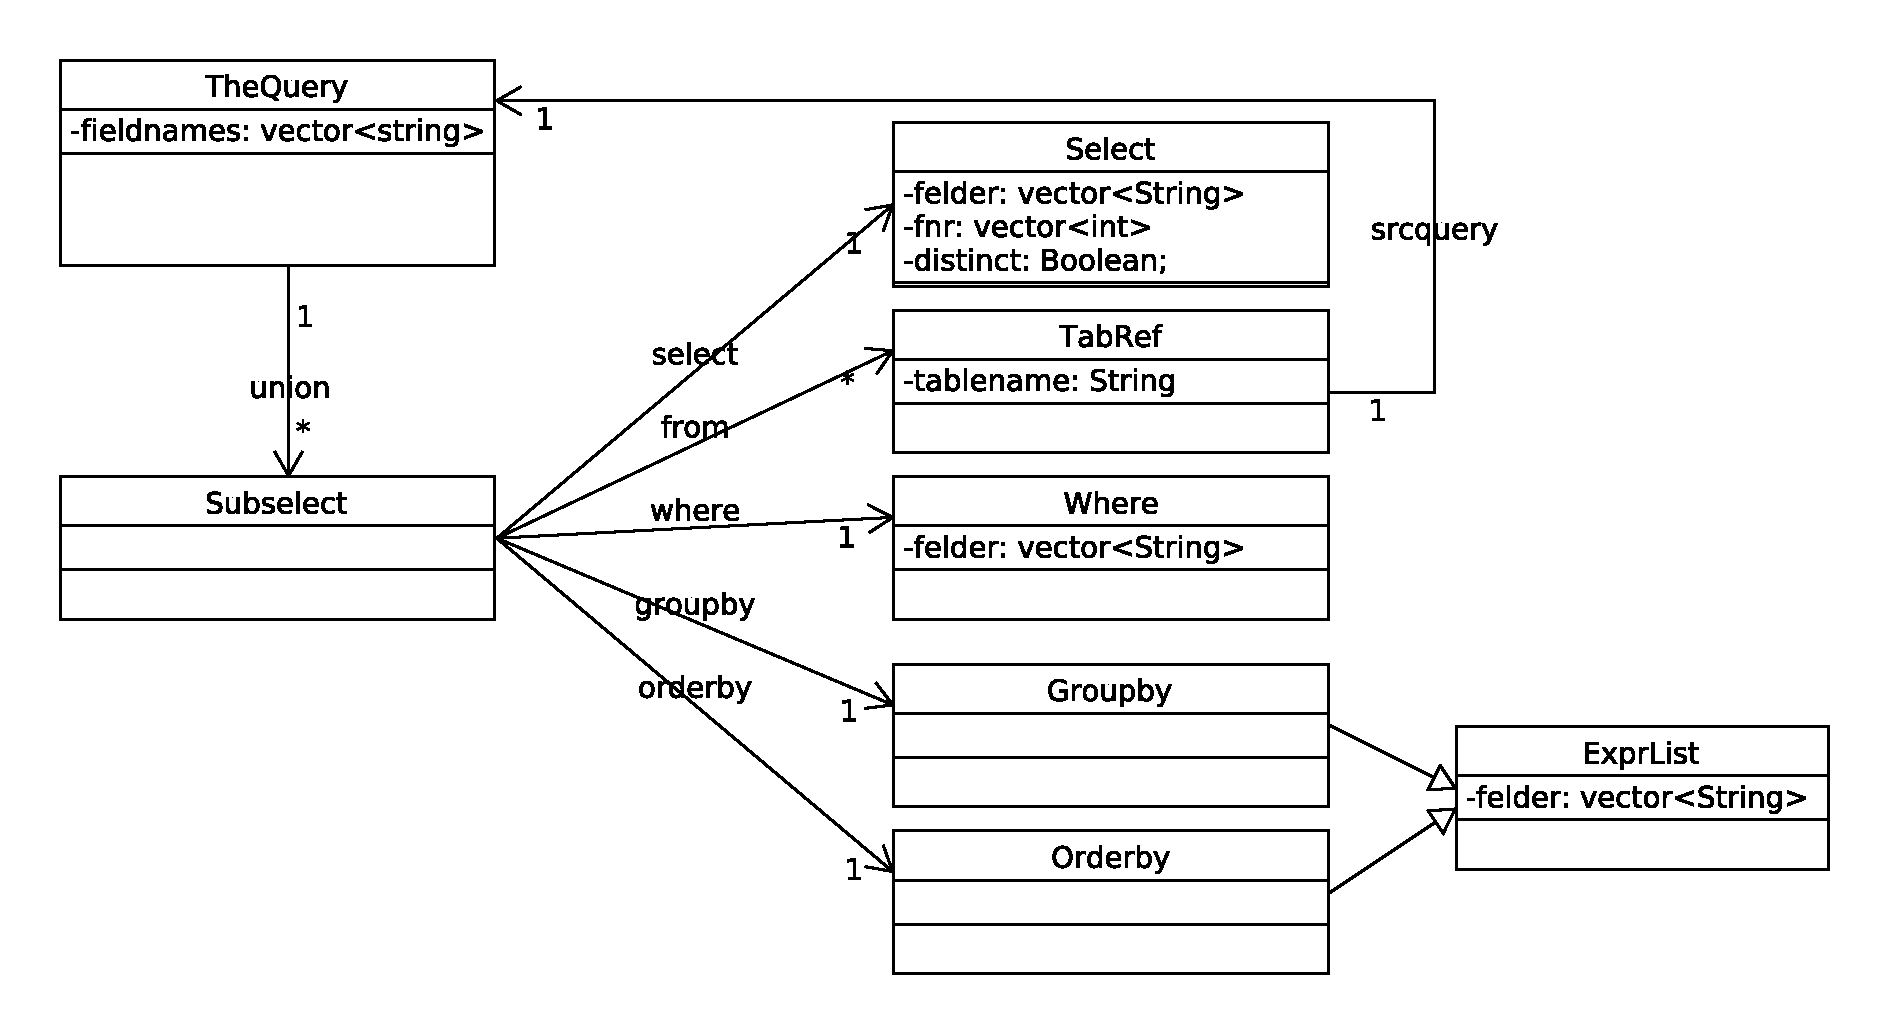
\includegraphics[scale=.4]{TheQuery.eps}
\caption{Aufbau der Klasse TheQuery}
\label{fig:TheQuery}
\end{figure}
Eine Klasse besteht aus einer Hauptklasse \textit{TheQuery}, die auch alle Methoden für den Zugriff kapselt (s. Abb. \ref{fig:TheQuery}). Sie verantwortet die Mengen aus mehreren eigentlichen Abfragen von \textit{Subselect} durch Vereinigung (vector<Subselect> union) oder auch die im Moment nicht benötigte Schnittmenge oder Differenz.
Die Klasse \textit{Subselect} bildet die eigentliche Abfrage mit einer \textit{Select}-Clause, einer Menge \textit{vector<TabRef> from} als Referenztabelle und den Objekten für Prädikate (\textit{Where}), Gruppierungen (\textit{Groupby}) und Sortierungen (\textit{Sortby}). Letztere beiden sind ähnlich als Vektor aus Feldern implementiert und erben noch von einer solchen Klasse \textit{ExprList}. Die Prädikate der Where-Klausel sind durch Konjunktionen (\textit{AND}) verknüpfte Aussagen und im Nachfolgenden wird eine konjunktive Normalform eingehalten, sodass eine Konjunktion aus Disjunktionen erstellt ist. In manchen Fällen wird als neutrales Element \textit{true} verwendet, wenn eine Aussage entfernt wird. Für Tabellen dient eine Klasse \textit{TabRef} mit einem Tabellennamen oder einer Referenz auf eine komplette Abfrage als Quelle. Die Referenz ist geeigneter als eine Vererbung, da die Klasse auch die textuelle Ausgabe mit einer entsprechenden Klammerung steuert.

\subsubsection{Darstellung der Felder}
Eine Schwierigkeit stellt die interne Repräsentation der Felder dar, da die Spaltenbezeichner nicht aus den Skripten hervorgehen und nicht davonauszugehen ist, das die Bezeichner aus einer Datei auszulesen sind. Deshalb werden vorübergehend die Feldbezeichner entsprechend zu awk gewählt (\textit{\$1,\$2,...}), das Maximum an Spalten muss dann definiert werden, wie gewohnt in \textit{MAXFIELDS}. Die gewählten Felder können direkt in die Select-Klausel eingefügt werden, auch als Zahlenvektor.

\begin{lstlisting}[language=C++]
void Select::addSelect(std::vector<int> feldnr)
{
        fnr=feldnr;
        /*copies values into felder*/
        for (std::vector<int>::iterator it = fnr.begin();
                it!=fnr.end(); it++){
                std::stringstream stmp;
                stmp << "$" << *it;
                felder.push_back(stmp.str());
        }
}
\end{lstlisting}

Alternativ können auch einzelne Feldbezeichner oder SQL-Ausdrücke wie Aggregatsfunktionen als Zeichenkette direkt eingegeben werden.
\begin{lstlisting}[language=C++]
void Select::addSelect(std::string name)
{
        felder.push_back(name);
}
\end{lstlisting}

Jedes Mal, wenn ein Tabellenname in die Abfrage eingelesen wird, wird überprüft, ob eine passende Datei mit passender Kopfzeile vorhanden ist, und mit der Methode \lstinline{getnamesfromfile()} werden die Spalten eingelesen, das Spaltentrennzeichen \textit{DELIMIT} wird durch den Präprozessor definiert.

\begin{lstlisting}[language=C++]
/*union more queries*/
void TheQuery::makeUnion(string src)
{
        /* table already defined? */
        if(queries[0]->notable())
                queries[0]->addTable(src);
        else
                queries.push_back(new Subselect(src));

        /*add column names*/
        getnamesfromfile(src,DELIMIT);
}
\end{lstlisting}

Die Methode \lstinline{getnamesfromfile()} setzt die Spaltennamen in \textit{fieldnames}, wenn noch nicht definiert, mit der Methode \lstinline{lookup()}. Diese Methode liest die erste Spalte einer Datei, trennt die Zeile nach dem Trennzeichen und gibt eine Vektor der Klasse String zurück.
\begin{lstlisting}[language=C++]
std::vector<std::string> TheQuery::lookup(std::string filename, char delimit)
{
        FILE *f;
        char * line = NULL;
        size_t len = 0;
        ssize_t read;
        char** ptr;
        std::vector<std::string> tmp;
        f=fopen(filename.c_str(),"r");
        if(!f)
                return std::vector<std::string>();
        if( read = getline(&line, &len, f) ==-1)
                return std::vector<std::string>();
        fclose(f);

        tmp=str_split(line,delimit);
        /* header columns terminated with delimiter symbol */
        tmp.pop_back();
        return tmp;
}
\end{lstlisting}

Das Attribut \textit{fieldnames} ist für das ganze Objekt einer Klasse \textit{TheQuery} gültig, da bei jeder Teilabfrage einer Vereinigung auch die Spaltenbezeichner identisch sein müssen. Bei Bildung eines Kreuzproduktes werden die hinzukommenden Spalten einfach hinzugefügt. Wird die Abfrage in einer anderen verwendet, so werden auch die Spaltennamen übergeben.

\begin{lstlisting}[language=C++]
void TheQuery::makeUnion(TheQuery* src)
{
        if(src==NULL)
                return;
        /* table already defined? */
        if(queries[0]->notable())
                queries[0]->addTable(src);
        else
                queries.push_back(new Subselect(src));
        /*get columnnames from file*/
        if(fieldnames.size()==0)
                fieldnames=src->getColumns();
}
\end{lstlisting}

Bevor eine Abfrage mit \textit{print()} ausgegeben wird, werden alle Hilfsspaltenbezeichner, die durch Dollar gekennzeichnet sind, ersetzt. Dazu stellt jede Klasse eine Methode \lstinline{replace_dollars()} zur Verfügung, die intern die Hilfsbezeichner ersetzt durch den passenden Spaltennamen aus \textit{fieldnames}.

\begin{lstlisting}[language=C++]
void TheQuery::print()
{
        /*only when a query is defined, should always be the case*/
        if(queries.size()>0){
                queries[0]->replace_dollars(fieldnames);
                queries[0]->print();
        }
        /* union all queries */
        for(int i=1; i<queries.size(); i++){
                std::cout << " UNION ";
                queries[i]->replace_dollars(fieldnames);
                /*now all unions must have an unique id*/
                queries[i]->print(i);
        }
}
\end{lstlisting}

Soweit steht die Klasse TheQuery und kann zur Erstellung der Abfragen genutzt werden, der Zugriff erfolgt nur über die Methoden von TheQuery, die auch im Anhnag zu finden sind.

\subsection{Der Parser näher betrachtet}
Der Übersetzer bzw. Compiler besteht aus zwei Teilen, zuerst wird der Syntax analysiert und ein Syntaxbaum generiert, dann können die zugehörigen Aktionen ausgeführt werden (vgl. Abbildung \ref{fig:parsen}). Dabei hat sich wenig verändert, die Syntaxanalyse funktionert in C++ etwas flexibler, manche Lexerregeln können besser gestaltet werden.

\begin{figure}[h]
\centering
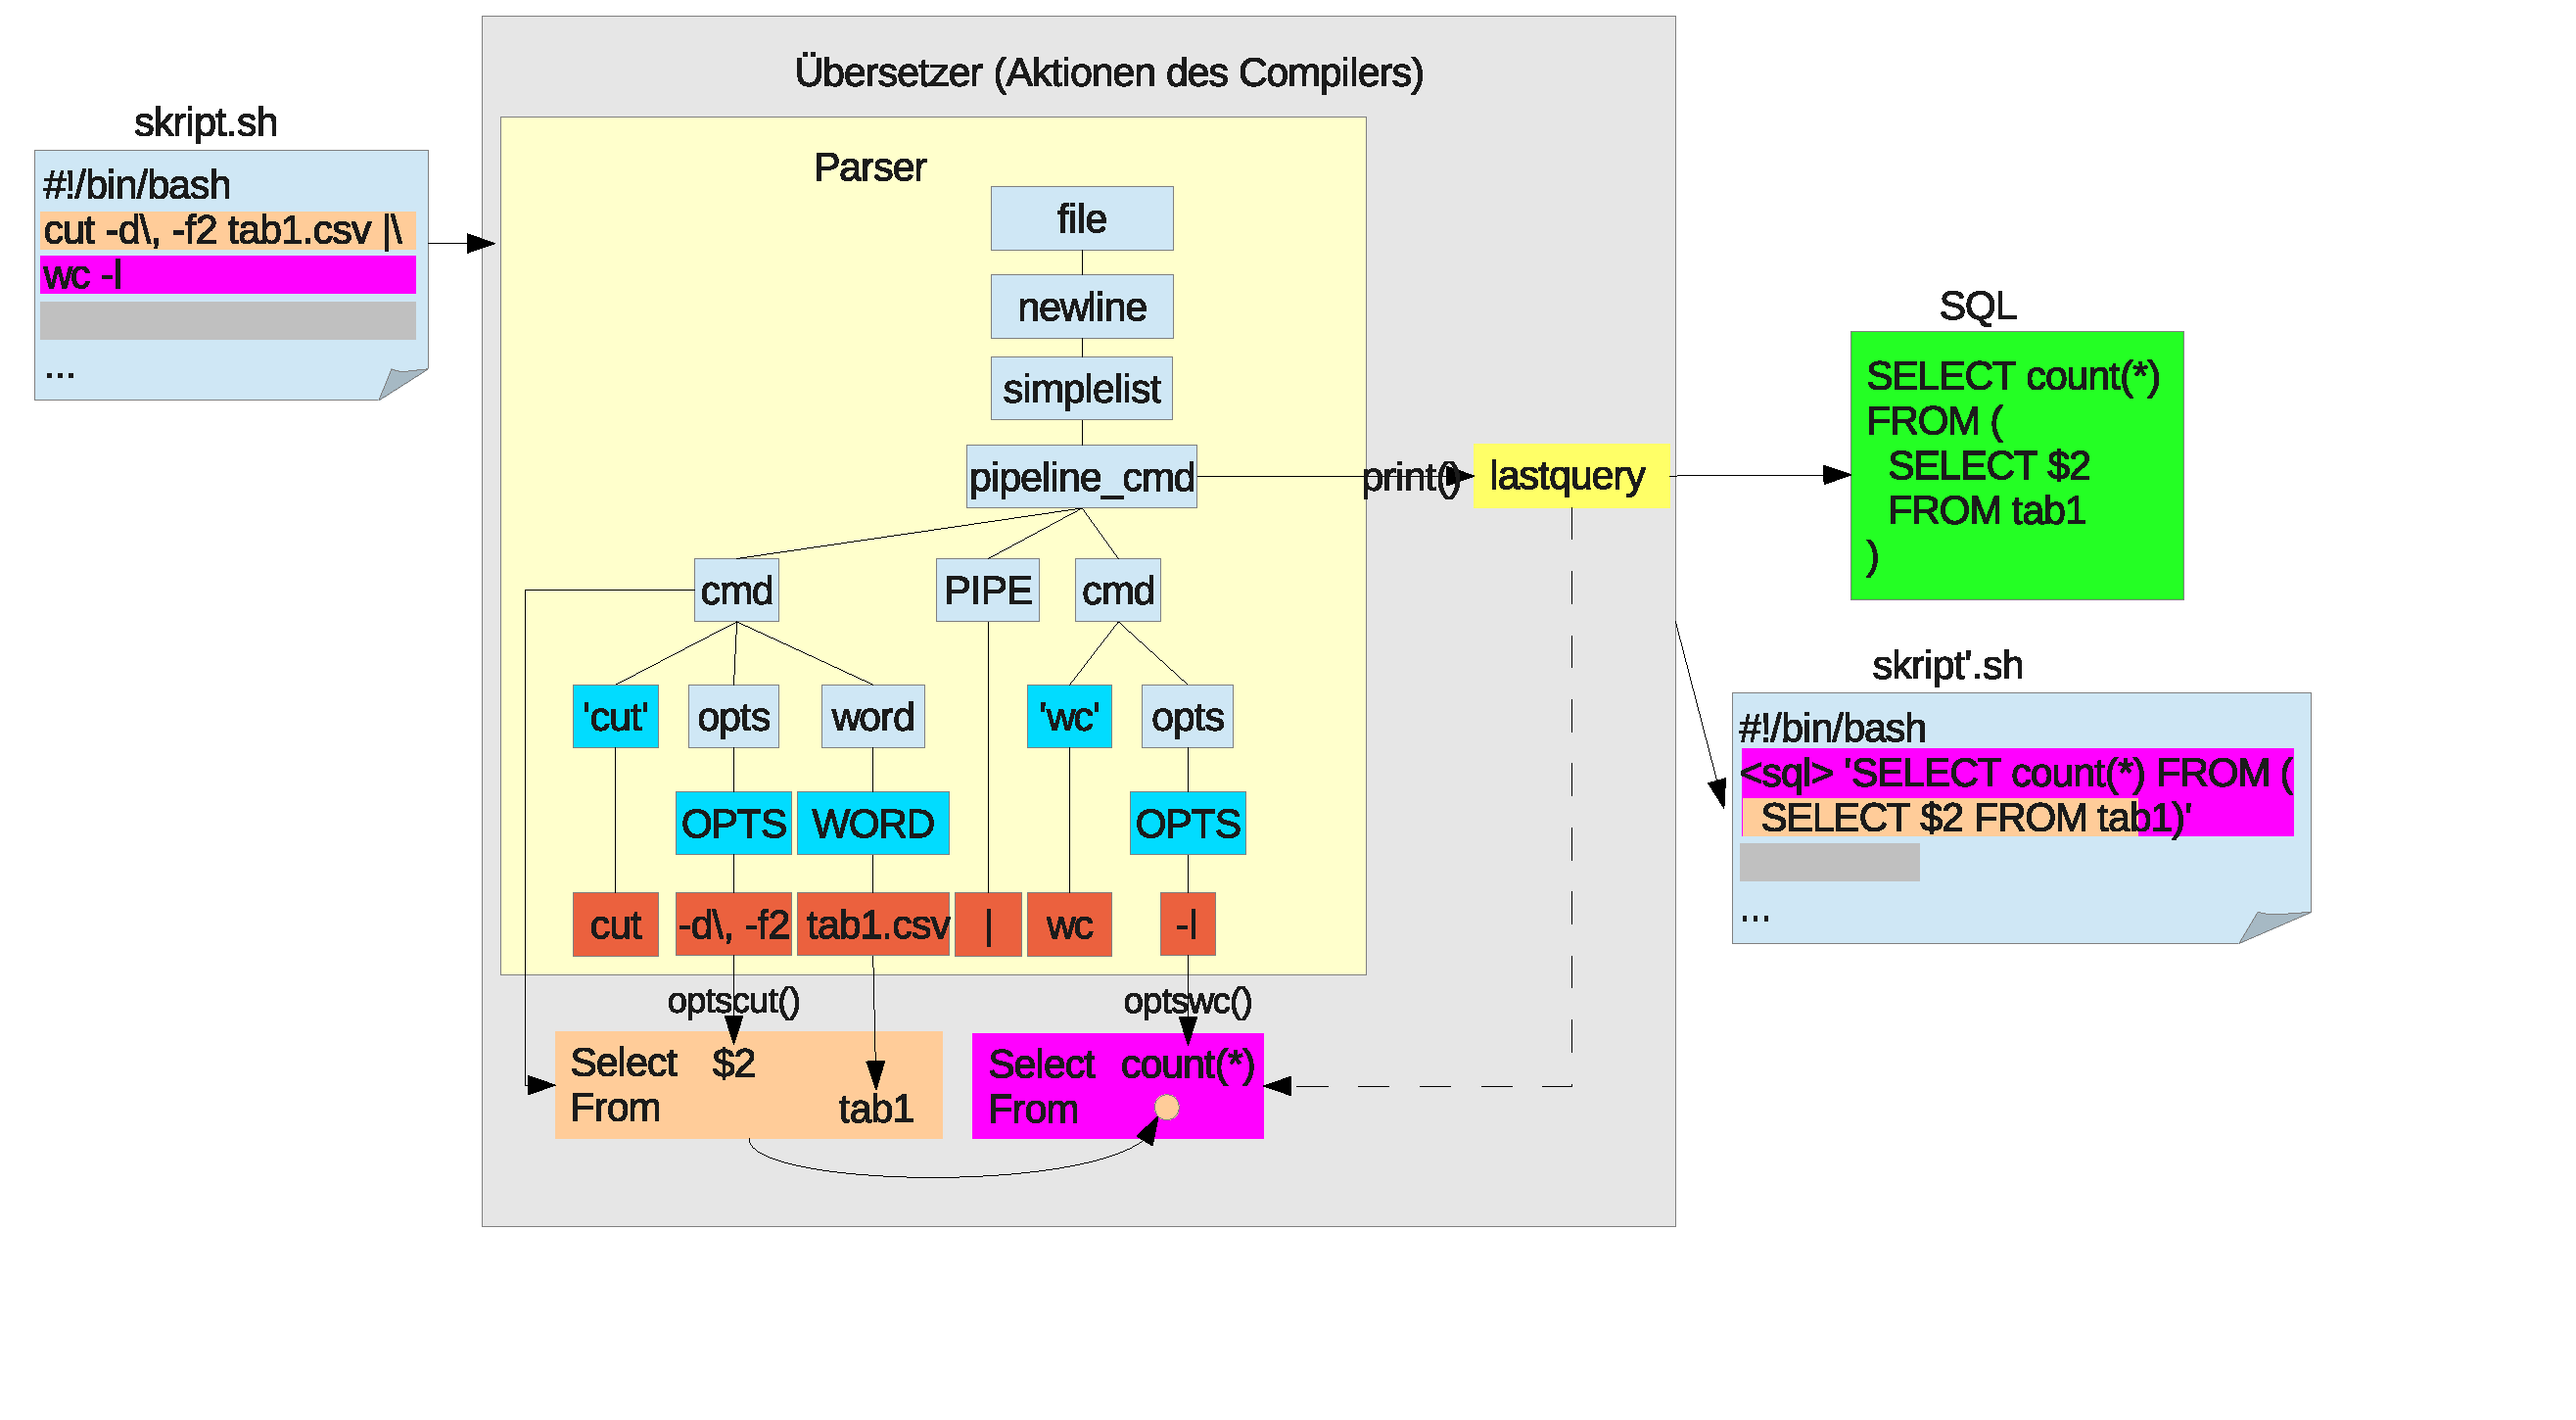
\includegraphics[scale=.4]{parsen.eps}
\caption{Parsen und Erstellen eine Syntaxbaums, anschließend Übersetzen}
\label{fig:parsen}
\end{figure}

Außerdem werden die Aktionen nun den Klassen angepasst, da die meiste Logik in \textit{cmd} passiert, nun ein kleiner Abriss:\\
Die Regel übernimmt zuerst die alte Abfrage, der Inhalt aus der Pipeline, also die zuletzt in SQL übersetzte Abfrage, also lastquery wird in einer temporären Variablen fromPipe gespeichert. Eine Subshell kann Teil einer Abfrage sein, deshalb wird lastquery auf NULL gesetzt, damit geöffnetete Subshells mit leerer Eingabe beginnen, also ohne einen Input. Anschließend kann eine neue SQL-Abfrage erzeugt werden, in die das zu parsende Kommando übersetzt wird. Alle weiteren Attribute dienen zur Bearbeitung bei bestimmten Kommandos (z.B. zählen der Argumente bei join), immer wird ein stringstream benötigt, in den der Inhalt der Symbole geschrieben wird. Am Ende der Regel wird die gerade erzeugte Abfrage als aktuelle gesetzt, also in die globale Variable lastquery.

\begin{lstlisting}[language=C++]
/* Rules for parsing bash command to SQL */
cmd returns [TheQuery *r]
@init{
        /* new TheQuery r,
        afterwards, set old query (lastquery) as table-reference
        set lastquery as null, so queries from subshell won't be
        included twice */
        TheQuery* fromPipe=lastquery;
        lastquery=NULL;
        r = new TheQuery();
        stringstream s;
        char buffer[80];
        int helpsize=0, join_on;
}
@after{
        /* query r is the most recent query  */
        lastquery=r;
}
\end{lstlisting}

\subsubsection{Das Kommando cut}
Da das Übersetzen der meisten Kommandos ähnlich erfolgt, wird nachfolgend wieder \textit{cut} vorgestellt (siehe auch Abb. \ref{fig:cut}).
\begin{lstlisting}[language=C++]
        :
          'cut'         ( opts
                                {
                                s.str(""); s.clear();
                                s << $opts.text; s.getline(buffer,80);
                                optscut(buffer,r);
                                }
                        | word
                                {
                                s.str(""); s.clear(); s << $word.text;
                                r->makeUnion(s.str());
                                }
                        | from_redir
                                {/* fname!=NULL, wenn Dateiname */
                                if (!$from_redir.fname.empty())
                                        r->makeUnion($from_redir.fname);
			          }
                        | '- '
                        )+
                        {r->makeUnion(fromPipe);}
\end{lstlisting}

Zuerst wird immer das Kommando abgefragt, anschließend werden die Parameter geparst, also Optionen, die Eingabe oder die Umlenkung als Eingabe. Für jedes Kommando muss eine eigene Regel erstellt werden. Die Aktionen zu den Regeln sind recht schlicht, die Optionen, über das Symbol \textit{opts}, das für alle Zeichenfolgen steht, die mit "'-"' eingeleitet werden, werden mit der zugehörigen Funktion \lstinline{optscut()} geparst und in die Abfrage übersetzt.
Als Parameter kann eine Quelldatei stehen, die als Tabellenname angenommen wird. Dies passiert mit der Methode der Klasse TheQuery \lstinline{makeUnion()}, die im Falle mehrerer Tabellen die Vereinigung darüber bildet.
Am Ende wird die über die Pipeline erhaltene Abfrage berücksichtigt, auch sie wird mit \lstinline{makeunion()} zur aktuellen Abfrage vereinigt.

\begin{figure}
\centering
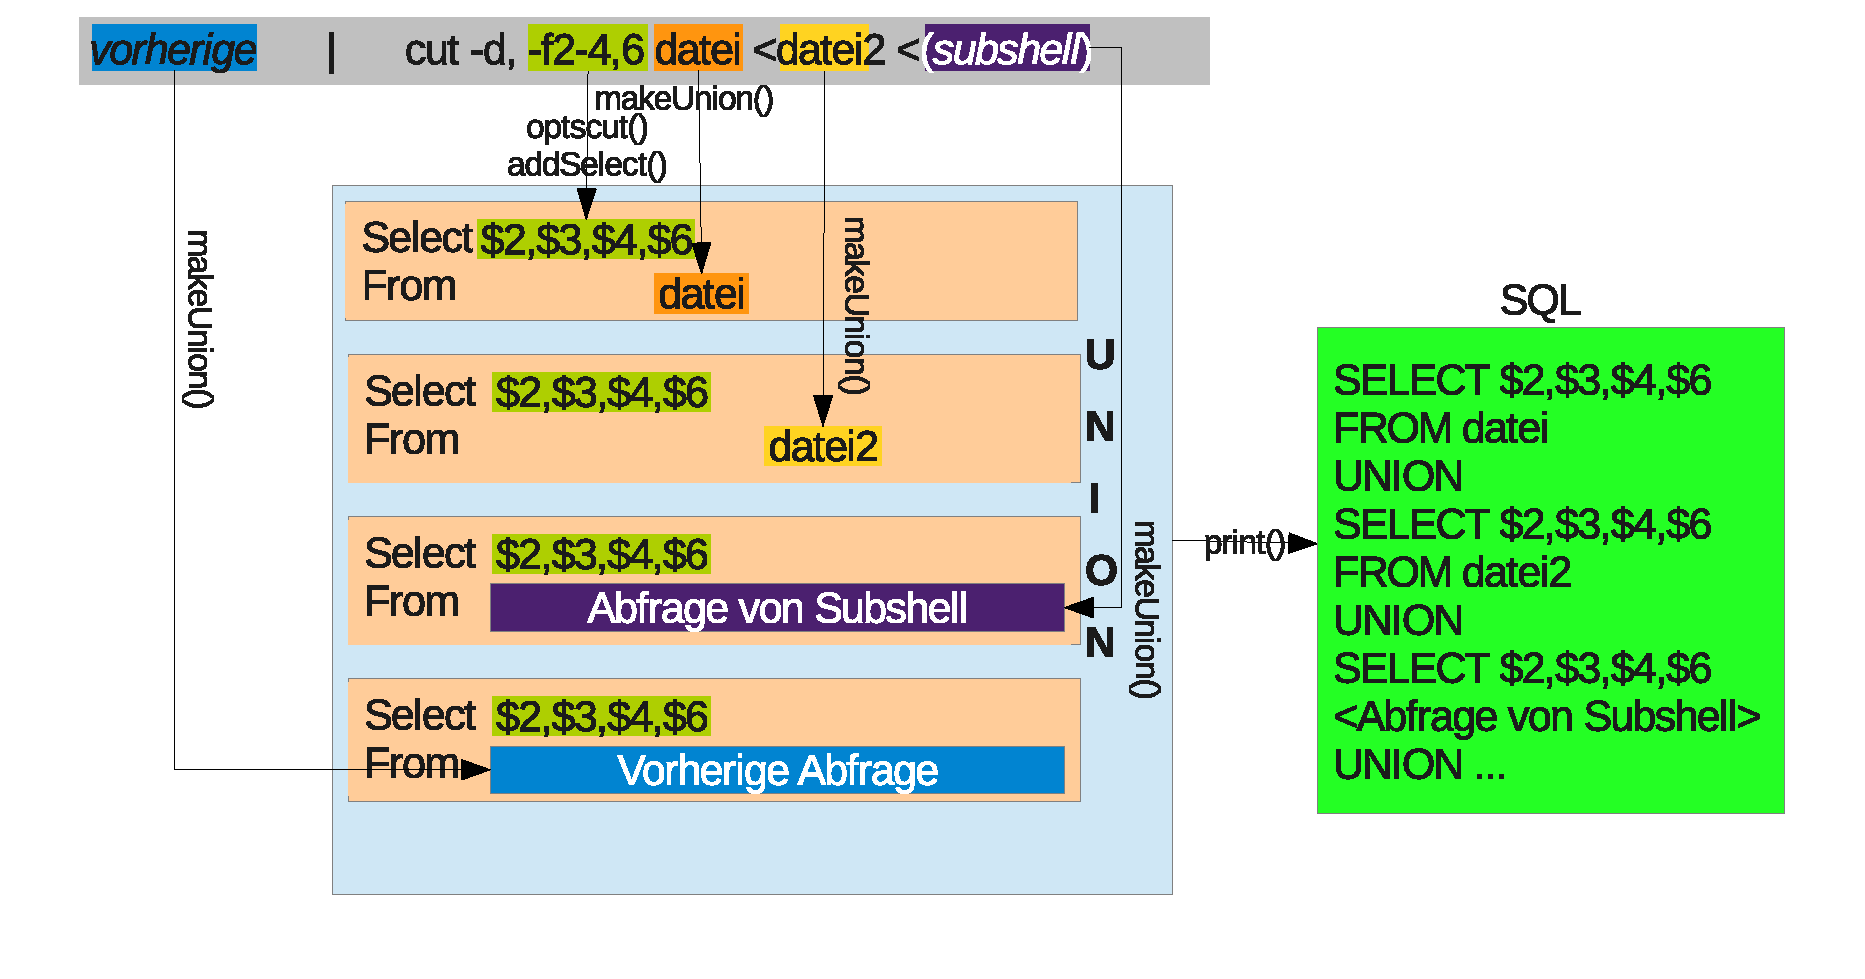
\includegraphics[scale=.4]{befehlcut.eps}
\caption{Konvertieren des Befehls cut in SQL}
\label{fig:cut}
\end{figure}

Das Vereinigen von Tabellen mittels \lstinline{makeUnion()} ist für fast alle Befehle identisch, auch das Parsen der Optionen ist meist sehr ähnlich, darum werden noch drei besondere Befehle hervorgehoben.

\subsubsection{Das Kommando grep}

\begin{figure}[h]
\centering
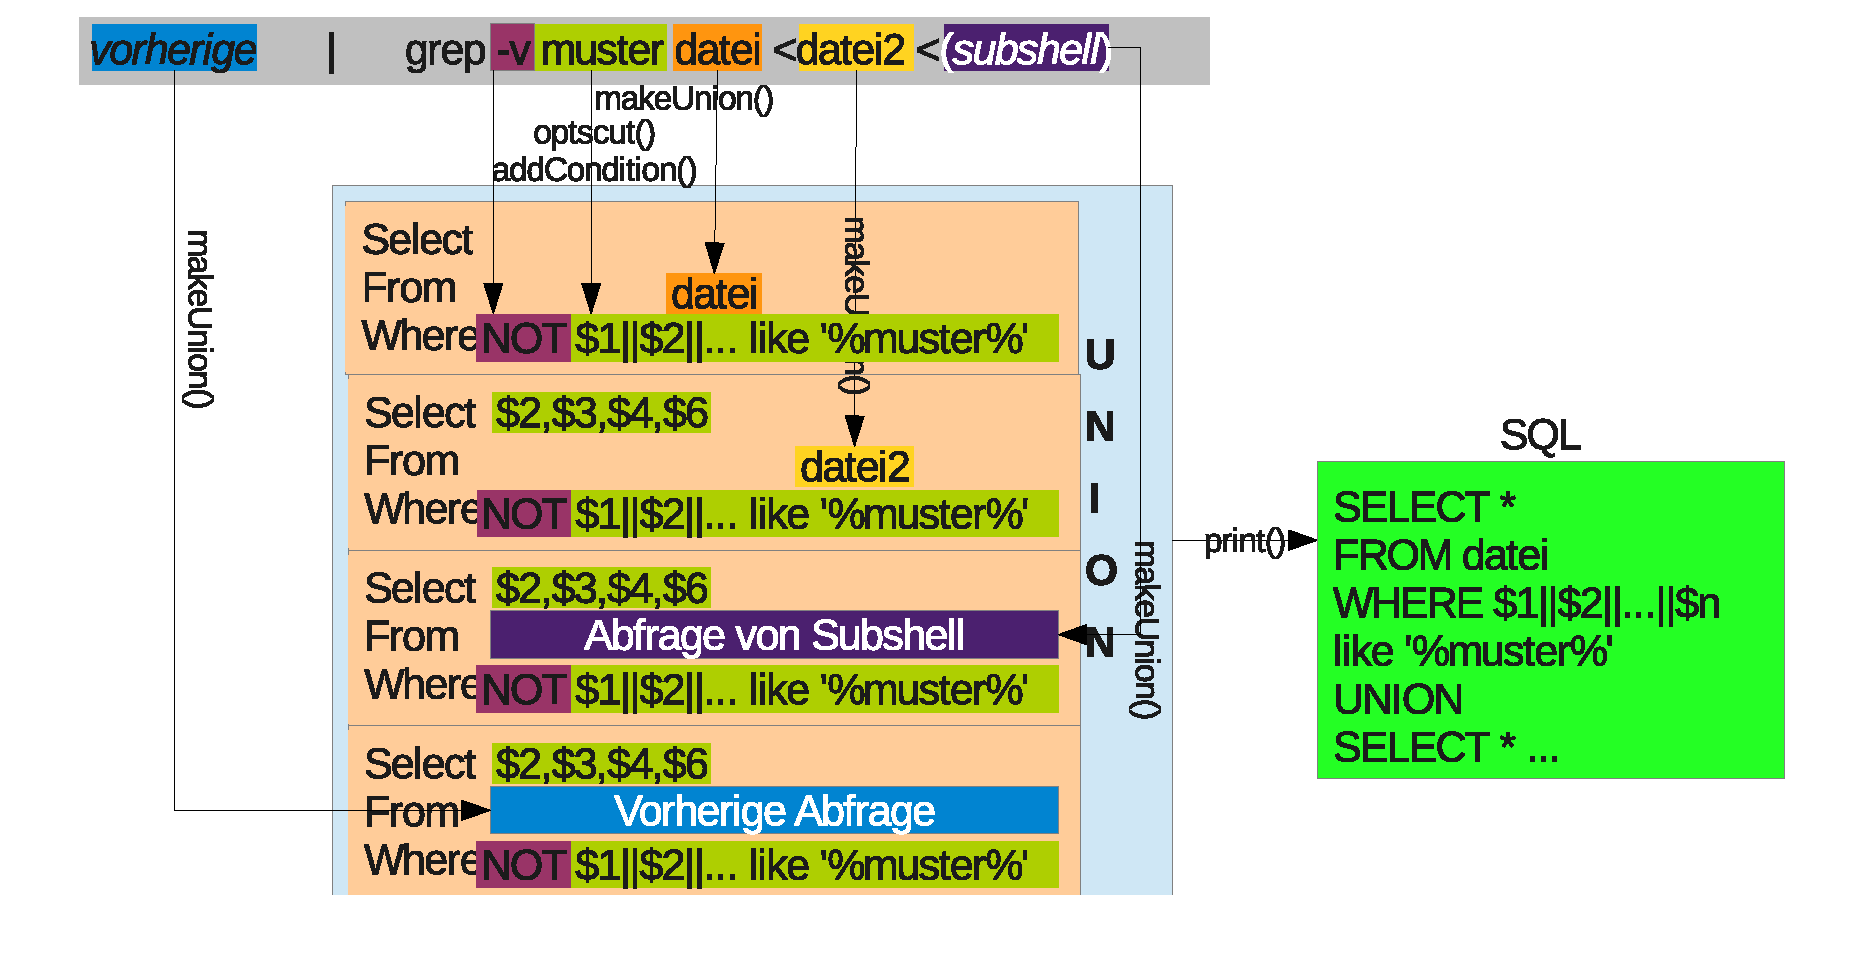
\includegraphics[scale=.4]{befehlgrep.eps}
\caption{Konvertieren des Befehls grep in SQL}
\label{fig:grep}
\end{figure}

Für den Befehl grep ist das angegebene Suchmuster mit allen Feldern zu vergleichen, daher werden zuerst alle Felder konkateniert (hier ist also die gesamte Anzahl an Spalten nötig) und danach wird mit \textit{like} nach Vorkommen des Musters darin gesucht. Da in grep eventuell auch das Spaltentrennzeichen mit angegeben ist, kann beim Verbinden der Felder auch das Zeichen berücksichtigt werden (\lstinline{$1||,||$2}).
Der erzeugte Ausdruck ist dabei in alle aktuellen Abfragen einzubinden.

\subsubsection{Das Kommando join}

\begin{figure}[h]
\centering
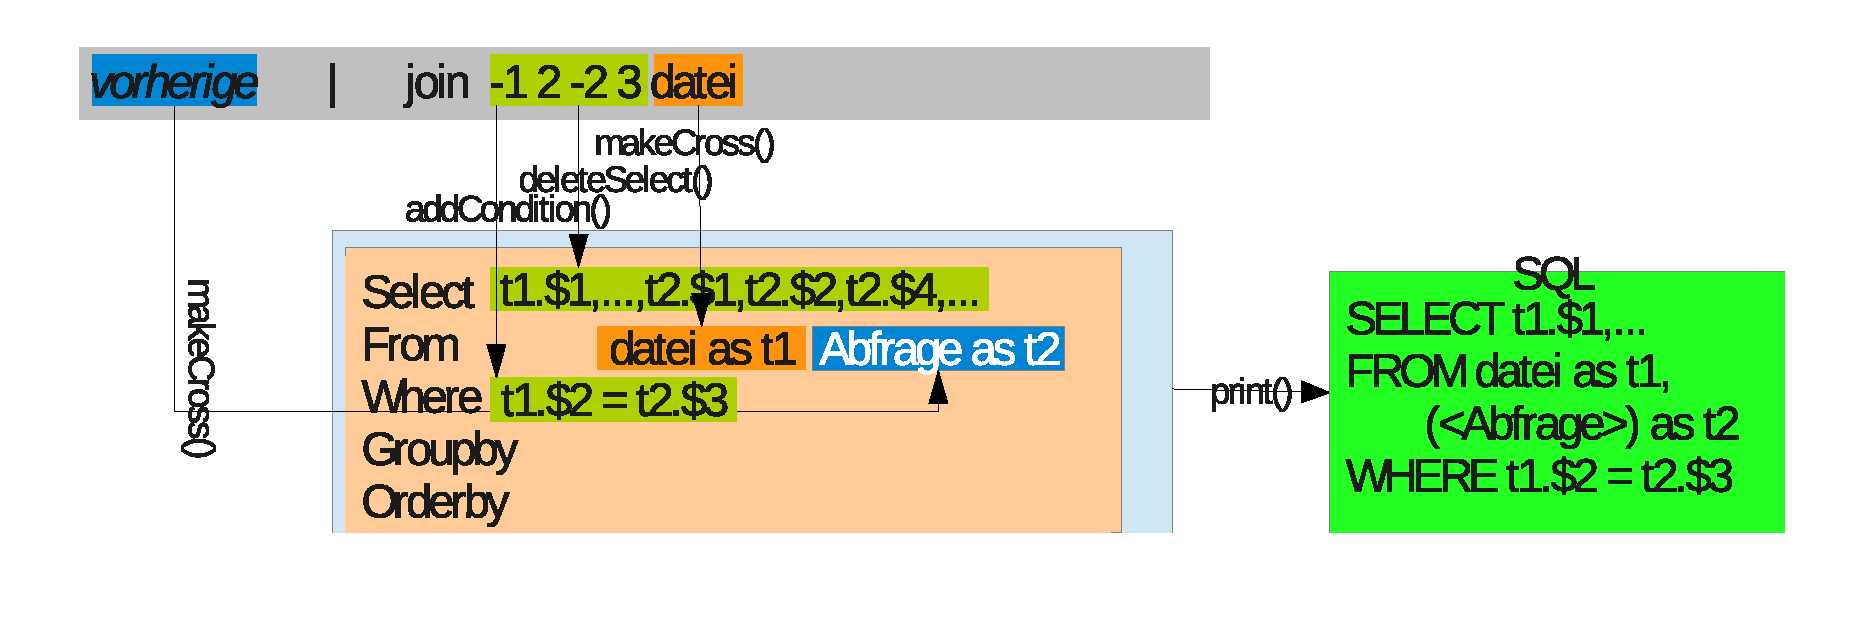
\includegraphics[scale=.4]{befehljoin.eps}
\caption{Konvertieren des Befehls join in SQL}
\label{fig:join}
\end{figure}

Den Verbund kann so in SQL übernommen werden, die zu verbindenden Spalten werden mit den Optionen \textit{-1} und \textit{-2} angegeben (ohne Angabe von Optionen wird über die jeweils erste Spalte verbunden), zu berücksichtigen ist noch die Reihenfolge der Tabellen, ob an erster oder zweiter Stelle, und dass die verbundene Spalte der zweiten Tabelle nicht im Ergebnis auftaucht. Um das Verbinden zu erleichtern, werden die beiden Tabellen noch mit einem Bezeichner versehen (t1, t2). Da keine Vereinigung sondern ein Join gebildet werden soll, erfolgt das Hinzufügen der Tabellen in die From-Klausel mittels \lstinline{makeCross()}.

\subsubsection{Ausdrücke der Sprache awk}

\begin{figure}[h]
\centering
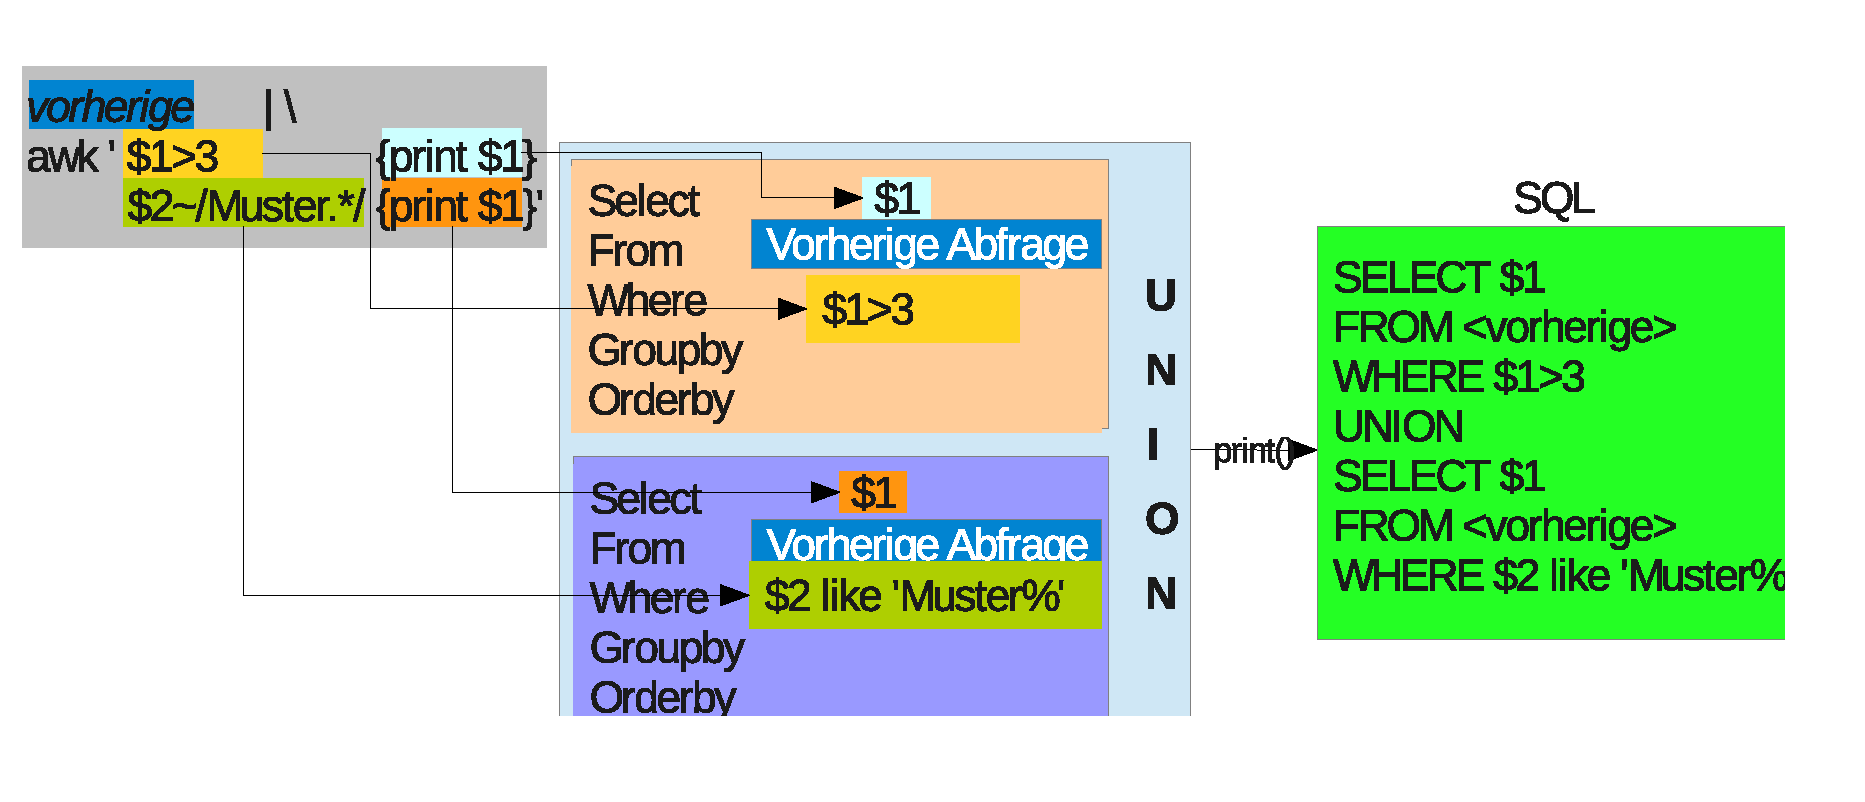
\includegraphics[scale=.4]{befehlawk.eps}
\caption{Konvertieren des Befehls awk in SQL}
\label{fig:awk}
\end{figure}

Das Programm übersetzt auch einfache Konstrukte der Sprache awk. Da sie meist aus einem Muster und einer folgenden Anweisung bestehen, kann das Muster als Bedingung und die Anweisung in die Select-Klausel übernommen werden. Besteht ein Suchmuster aus einem einfachen Vergleich wie
\lstinline{$2 == "Inhalt"},
so kann das Muster direkt in die Bedingung übernommen werden, lediglich die Kennzeichnung von Zeichenketten durch einfache Hochkommata und die Äquivalenz durch ein einfaches "'="' müssen angepasst werden (\lstinline{$2 = 'Inhalt'}). Reguläre Ausdrucke sind ähnlich anzupassen (\lstinline{$2 ~/.Muster.*/}), da sie, identisch zu grep, dem \textit{like}-Operator entsprechen (\lstinline{$2 like '?Muster\%'}).
Da nach jedem Muster eine andere Aktion folgt, sind diese auch als unabhängige Anfragen zu betrachten, für jedes Muster muss eine erneute Abfrage desselben Ursprungs mit identischen From-Klauseln erstellt werden. In die Select-Klausel wird jedes \lstinline{print} übersetzt, denn nur da erfolgt eine Ausgabe. Im Moment werden nur Ausgaben der Felder unterstützt wie \lstinline{print $1, $2}, kompliziertere arithmetische Ausdrücke und Ausgabe von Variablen müssten in eine entsprechende Anweisung mit \textit{case} umgewandelt werden.

\subsection{Bedienung}
Im Ordner \textit{plus\_bash\_parser\_yacc} liegen die Grammatikdatei \textit{SimpleBashSQL.g}, die Dateien TheQuery.hpp und -.cpp, eine dynamische Bibliothek und ein Makefile. Wie im vorherigen Fall wird der Compiler automatisch generiert, wenn die Konfiguration richtig erfolgt ist. Alternativ kann das init-Skript angepasst werden, das die Pfade richtig setzt.
\begin{lstlisting}[language=Bash]
$ . ./init
\end{lstlisting}

ANTLR erzeugt eine Lexer- und eine Parser-Quelldatei \textit{SimpleBashSQL\{Lexer,Parser\}.\{hpp,cpp\}}, die zu dem fertigen Compiler mittels \textit{g++} kompiliert werden.

\begin{lstlisting}[language=make]
simplebashsql: theparser thequery.o
        g++ -std=c++11 -g -o $@ $(CFLAGS) -lantlr3c $(OBJ)Parser.cpp $(OBJ)Lexer.cpp thequery.o
        rm thequery.o
\end{lstlisting}

Das Programm nimmt den Dateinamen eines Skripts als Eingabeparameter und schickt das Ergebnis auf die Standardausgabe. So wird das Skript:
\begin{lstlisting}[language=Bash]
$ cat testskript.sh
#!/bin/bash
cut -f1,2,3 vorlesungen.csv | sort -k2
\end{lstlisting}
übersetzt in:
\begin{lstlisting}[language=Bash]
$ ./simplebashsql testskript.sh
SELECT * FROM (SELECT $1,$2,$3 FROM vorlesungen.csv as t1 ) as t1  ORDER BY $2
\end{lstlisting}

Existiert darüber hinaus eine Datei vorlesungen.csv mit Kopfzeile, so erkennt das Programm gleich die Spaltenbezeichner und erzeugt sprechende Namen.
\begin{lstlisting}[language=Bash]
$ head -1 vorlesungen.csv
VorlNr,Titel,SWS,
$ ./simplebashsql testskript.sh
SELECT * FROM (SELECT VorlNr,Titel,SWS FROM vorlesungen.csv as t1 ) as t1  ORDER BY Titel
\end{lstlisting}

\subsection{Rückübersetzung einer TPC-H Abfrage}
Um wieder zu den TPC-H Abfragen zurückzukehren, so genügen die definierten Regeln um die anfangs beschriebene vierte Abfrage wieder zurückzuübersetzen.
\begin{lstlisting}[language=Bash]
$ ./simplebashsql query4b
mkfifo tmporder.csv
WITH tmporder.csv AS (
SELECT $1,$6 FROM (SELECT * FROM orders.csv as t1  UNION SELECT * FROM (SELECT * FROM orders.tbl as t1  ORDER BY $1,$1) as t1union1 ) as t1  WHERE (true) AND ($5<'1993-10-01') AND ($5>='1993-07-01')  )

WITH tmpline.csv AS (
SELECT $1 FROM (SELECT $1 FROM (SELECT * FROM lineitem.csv as t1  UNION SELECT * FROM (SELECT * FROM lineitem.tbl as t1  ORDER BY $1,$1) as t1union1 ) as t1  WHERE (true) AND ($12<$13) ) as t1  GROUP BY $1 )

SELECT count(*),$2 FROM (SELECT * FROM (SELECT * FROM (SELECT $2 FROM (SELECT $1,$2,$3,$4,$5,$6,$7,$8,$9 FROM tmporder.csv as t1, tmpline.csv as t2  WHERE (t1.$1=t2.$10) ) as t1 ) as t1 ) as t1 ) as t1  GROUP BY $2
rm tmp*.csv
\end{lstlisting}

Im Moment erscheinen noch kryptische Spaltenbezeichner, denn die Dateien konnten noch nicht gefunden werden, der Übersetzer nimmt für jede Tabelle die definierten neun Spalten an. Für jede eingelesene Datei muss jetzt eine Datei mit Kopfzeilen definiert sein, für Abfragen innerhalb einer Vereinigung genügt die Existenz einer Datei mit Kopfzeilen (orders.csv gibt für orders.tbl mit die Spalten an). Leider erzeugt das Programm noch keine solche Datei für Hilfstabellen, die das Skript erzeugt. Folglich müssen für tmporder.csv und tmpline.csv auch Dateien hinterlegt werden (das ursprüngliche Skript ist ausgeführt worden um an die Dateien zu gelangen).
\begin{lstlisting}[language=Bash]
$ cat orders.csv 
o_orderkey,o_custkey,o_orderstatus,o_totalprice,o_orderdate,o_orderpriority,o_clerk,o_shippriority,o_comment,
$ cat orders.csv 
o_orderkey,o_custkey,o_orderstatus,o_totalprice,o_orderdate,o_orderpriority,o_clerk,o_shippriority,o_comment,
$ cat lineitem.csv 
l_orderkey,l_partkey,l_suppkey,l_linenumber,l_quantity,l_extendedprice,l_discount,l_tax,l_returnflag,l_linestatus,l_shipdate,l_commitdate,l_receiptdate,l_shipinstruct,l_shipmode,l_comment,
$ cat tmporder.csv 
o_orderkey,o_orderpriority,
$ cat tmpline.csv 
l_orderkey,
$ ./simplebashsql query4b
\end{lstlisting}\begin{lstlisting}[language=SQL]
mkfifo tmporder.csv
WITH tmporder.csv AS (
SELECT o_orderkey,o_orderpriority FROM (SELECT * FROM orders.csv as t1  UNION SELECT * FROM (SELECT * FROM orders.tbl as t1  ORDER BY $1,$1) as t1union1 ) as t1  WHERE (true) AND (o_orderdate<'1993-10-01') AND (o_orderdate>='1993-07-01')  )

WITH tmpline.csv AS (
SELECT l_orderkey FROM (SELECT l_orderkey FROM (SELECT * FROM lineitem.csv as t1  UNION SELECT * FROM (SELECT * FROM lineitem.tbl as t1  ORDER BY $1,$1) as t1union1 ) as t1  WHERE (true) AND (l_commitdate<l_receiptdate) ) as t1  GROUP BY l_orderkey )

SELECT count(*),o_orderpriority FROM (SELECT * FROM (SELECT * FROM (SELECT o_orderpriority FROM (SELECT o_orderkey,o_orderpriority FROM tmporder.csv as t1, tmpline.csv as t2  WHERE (t1.o_orderkey=t2.l_orderkey) ) as t1 ) as t1 ) as t1 ) as t1  GROUP BY o_orderpriority
rm tmp*.csv
\end{lstlisting}

Diese Abfrage kann nun über eine SQL-Schnittstelle eingegeben werden, vorher müssen die Dateiendungen entfernt werden (.csv), die manche SQL-Inline-Tools jedoch benötigen, anschließend kann die Zeit gemessen werden.% (s. Abb. \ref{Zeit}).
%\begin{figure}

\begin{center}
\begin{tabular}{|l|r|}
Abfrage & Zeit \\ \hline
Query4 original & 62.87\ ms\\
Query4b Skript &  21\ 910,00\ ms\\
Query4b rückübersetzt & 5\ 946.87\ ms
\end{tabular}
%\caption{gemessene Zeiten im Vergleich}
%\label{fig:Zeit}
%\end{figure}
\end{center}
